\chapter{Multimodal face-evoked responses \label{Chap:data:multimodal}}

\section{Overview}

This dataset contains EEG, MEG, functional MRI and structural MRI data on the same subject with the same paradigm, which allows a basic comparison of faces versus scrambled faces.

It can be used to demonstrate, for example, 3D source reconstruction of various electrophysiological measures of face perception, such as the ``N170'' evoked response (ERP) recorded with EEG, or the analogous ``M170'' evoked field (ERF) recorded with MEG. These localisations are informed by the anatomy of the brain (from the structural MRI) and possibly by functional activation in the same paradigm (from the functional MRI).

The demonstration below involves localising the N170 using a distributed source method (called an ``imaging'' solution in SPM). The data can also be used to explore further effects, e.g. induced effects (Friston et al, 2006), effects at different latencies, or the effects of adding fMRI constraints on the localisation.

The EEG data were acquired on a 128 channel ActiveTwo system; the MEG data were acquired on a 275 channel CTF/VSM system; the sMRI data were acquired using a phased-array headcoil on a Siemens Sonata 1.5T; the fMRI data were acquired using a gradient-echo EPI sequence on the Sonata. The dataset also includes data from a Polhemus digitizer, which are used to coregister the EEG and the MEG data with the structural MRI.

Some related analyses of these data are reported in Henson et al (2005a, 2005b, 2007, 2009a, 2009b, under revision), Kiebel and Friston (2004) and Friston et al (2006). To proceed with the data analysis, first download the  data set from the SPM website\footnote{Multimodal face-evoked dataset: \url{http://www.fil.ion.ucl.ac.uk/spm/data/mmfaces/}}.
Most of the analysis below can be implemented in \matlab\ 7.1 (R14SP3) and above. However, recoding condition labels using the GUI requires features of SPM8 only available in \matlab\ 7.4 (R2007a) and above. The Signal Processing toolbox is required for the filtering and downsampling steps.

\section{Paradigm and Data}

The basic paradigm involves randomised presentation of at least 86 faces and 86 scrambled faces (Figure~\ref{multimodal:fig:1}), based on Phase 1 of a previous study by Henson et al (2003). The scrambled faces were created by 2D Fourier transformation, random phase permutation, inverse transformation and outline-masking of each face. Thus faces and scrambled faces are closely matched for low-level visual properties such as spatial frequency content. Half the faces were famous, but this factor is collapsed in the current analyses. Each face required a four-way, left-right symmetry judgment (mean RTs over a second; judgments roughly orthogonal to conditions; reasons for this task are explained in Henson et al, 2003). The subject was instructed not to blink while the fixation cross was present on the screen.

\begin{figure}
\begin{center}
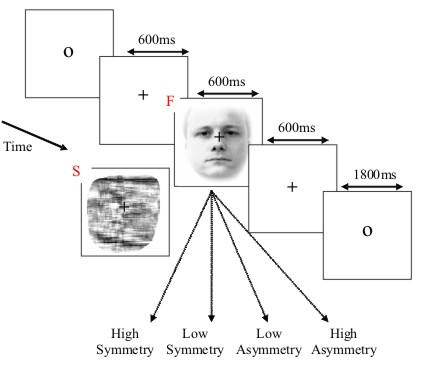
\includegraphics[width=100mm]{multimodal/figures/paradigm}
\caption{\em One trial in the experiment. Trials involved either a Face (F) or Scrambled face (S). \label{multimodal:fig:1}}
\end{center}
\end{figure}

\subsection{Structural MRI}

The T1-weighted structural MRI of a young male was acquired on a 1.5T Siemens Sonata via an MDEFT sequence with resolution $1 \times 1 \times 1 mm^3$ voxels, using a whole-body coil for RF transmission and an 8-element phased array head coil for signal reception.

The images are in Analyze format in the sMRI sub-directory, consisting of two files:
\begin{verbatim}
    sMRI/sMRI.img
    sMRI/sMRI.hdr
\end{verbatim}
The structural was manually-positioned to roughly match Talairach space, with the origin close to the Anterior Commissure, which produced the associated SPM \matlab\ file:
\begin{verbatim}
    sMRI/sMRI.mat
\end{verbatim}
The approximate position of 3 fiducials within this MRI space - the nasion, and the left and right peri-aricular points - are stored in the file:
\begin{verbatim}
    sMRI/smri_fid.txt
\end{verbatim}
These were identified manually (based on anatomy) and are used to define the MRI space relative to the EEG and MEG spaces, which need to be coregistered (see below). It doesn't matter that the positions are approximate, because more precise coregistration is implemented via digitised surfaces of the scalp (``head shape functions'') that were created using the Polhemus 3D digitizer.

\subsection{EEG data}

The EEG data were acquired on a 128-channel ActiveTwo system, sampled at 2048 Hz, plus electrodes on left earlobe, right earlobe, and two bipolar channels to measure HEOG and VEOG. The 128 scalp channels are named: 32 A (Back), 32 B (Right), 32 C (Front) and 32 D (Left). The data acquired in two runs of the protocol are contained in two Biosemi raw data files:
\begin{verbatim}
    EEG/faces_run1.bdf
    EEG/faces_run2.bdf
\end{verbatim}

The EEG directory also contains the following files:
\begin{verbatim}
    EEG/condition_labels.txt
\end{verbatim}
This text file contains a list of condition labels in the same order as the trials appear in the two files - ``faces'' for presentation of faces and ``scrambled'' for presentation of scrambled faces.
The EEG directory also contains the following files:
\begin{verbatim}
    EEG/electrode_locations_and_headshape.sfp
\end{verbatim}
This ASCII file contains electrode locations, fiducials and headshape points measured with Polhemus digitizer.

The 3 fiducial markers were placed approximately on the nasion and preauricular points and digitised by the Polhemus digitizer.  Later, we will coregister the fiducial points and the head shape to map the electrode positions in the ``Polhemus space'' to the ``MRI space''.
Also included as reference are some SPM batch files and SPM scripts (though these are recreated as part of the demo):

\begin{verbatim}
    EEG/batch_eeg_XYTstats.mat
    EEG/batch_eeg_artefact.mat
    EEG/eeg_preprocess.m
    EEG/faces_eeg_montage.m
\end{verbatim}


\subsection{MEG data}

The MEG data were acquired on a 275 channel CTF/VSM system, using second-order axial gradiometers and synthetic third gradient for denoising and sampled at 480 Hz. There are actually 274 MEG channels in this dataset since the system it was recorded on had one faulty sensor. Two runs (sessions) of the protocol have been saved in two CTF datasets (each one is a directory with multiple files) 
\begin{verbatim}
    MEG/SPM_CTF_MEG_example_faces1_3D.ds
    MEG/SPM_CTF_MEG_example_faces2_3D.ds
\end{verbatim}
The MEG data also contains a \texttt{headshape.mat} file, containing the headshape recorded during the MEG experiment with a Polhemus digitizer.

The locations of the 3 fiducials in the \texttt{headshape.mat} file are the same as the positions of 3 ``locator coils'' the locations of which are measured by the CTF machine, and used to define the coordinates (in ``CTF space'') for the location of the 275 sensors.

Also included as reference are two SPM batch files and two trial definition files (though these are recreated as part of the demo):
\begin{verbatim}
    MEG/batch_meg_preprocess.mat
    MEG/batch_meg_TFstats.mat
    MEG/trials_run1.mat
    MEG/trials_run2.mat
\end{verbatim}

\subsection{fMRI data}

The fMRI data were acquired using a gradient-echo EPI sequence on a 3T Siemens TIM Trio, with 32, 3mm slices (skip 0.75mm) of $3\times 3 mm^2$ pixels, acquired in a sequential descending order with a TR of 2s. There are 390 images in each of the two ``Session'' sub-directories (5 initial dummy scans have been removed), each consisting of an Analyze image and header file:
\begin{verbatim}
    fMRI/Session1/fM*.{hdr,img}
    fMRI/Session2/fM*.{hdr,img}
\end{verbatim}
Also provided are the onsets of faces and scrambled faces (in units of scans) in the \matlab\ file:
\begin{verbatim}
    fMRI/trials_ses1.mat
    fMRI/trials_ses2.mat
\end{verbatim}
and two example SPM batch files (see Section~\ref{multimodal:data:fMRI}):
\begin{verbatim}
    fMRI/batch_fmri_preproc.mat
    fMRI/batch_fmri_stats.mat
\end{verbatim}


\section{Getting Started}

You need to start SPM8 and toggle ``EEG'' as the modality (bottom-right of SPM main window), or start SPM8 with \texttt{spm eeg}. In order for this to work you need to ensure that the main SPM directory is on your \matlab\ path.

\section{EEG analysis \label{multimodal:data:eeg}}

First change directory to the EEG subdirectory (either in \matlab\, or via the ``CD'' option in the SPM ``Utils'' menu).

\subsection{Convert}

Press the \textsc{Convert} button and select the \texttt{faces\_run1.bdf} file. At the prompt ``Define settings?'' select ``just read''.
SPM will now read the original Biosemi format file and create an SPM compatible data file, called \texttt{spm8\_faces\_run1.mat} and \texttt{spm8\_faces\_run1.dat} in the current \matlab\ directory. After the conversion is complete the data file will be automatically opened in SPM8 reviewing tool. By default you will see the ``info'' tab. At the top of the window there is some basic information about the file. Below it you will see several clickable tabs with additional information. The ``history'' tab lists the processing steps that have been applied to the file. At this stage there is only one such step - conversion. The ``channels'' tab lists the channels in the file and their properties, the ``trial'' tab lists the trials or in the case of a continuous file all the triggers (events) that have been recorded. The ``inv'' tab is used for reviewing the inverse solutions and is not relevant for the time being. Note that the detailed information in the tabs will not be available for \matlab\ versions older than 7.4.  At the top of the window there is another set of tabs. If you click on the ``EEG'' tab you will see the raw EEG traces. They all look unusually flat because the continuous data we have just converted contains very low frequencies and baseline shifts. Therefore, if we try to view all the channels together, this can only be done with very low gain.
If you press the ``intensity rescaling'' button (with arrows pointing up and down) several times you will start seeing EEG activity in a few channels but the other channels will not be visible as they will go out of range. You can also use the controls at the bottom of the window to scroll through the recording. If you press the icon to the right of the mini-topography icon, with the rightwards pointing arrow, the display will move to the next trigger, shown as a vertical line through the display. (New triggers/events can be added by the rightmost icon). At the bottom of the display is a plot of the global field power across the session, with the black line indicating the current timewindow displayed (the width of this timewindow can be controlled by the two leftmost top icons).

\subsection{Downsample}

Here, we will downsample the data in time. This is useful when the data were acquired like ours with a high sampling rate of 2048 Hz. This is an unnecessarily high sampling rate for a simple evoked response analysis, and we will now decrease the sampling rate to 200 Hz, thereby reducing the file size by more than ten fold and greatly speeding up the subsequent processing steps. This step requires the Signal Processing toolbox. Select \textsc{Downsample} from the ``Other'' drop-down menu and select the \texttt{spm8\_faces\_run1.mat} file. Choose a new sampling rate of 200 (Hz). The progress bar will appear and the resulting data will be saved to files \texttt{dspm8\_faces\_run1.mat} and \texttt{dspm8\_faces\_run1.dat}. Note that this dataset and other intermediate datasets created during preprocessing will not be automatically opened in the reviewing tool, but you can always review them by selecting \texttt{M/EEG} from the ``Display'' drop down menu and choosing the corresponding \texttt{.mat} file.

\subsection{Montage}

In this step, we will identify the VEOG and HEOG channels, remove several channels that don't carry EEG data and are of no importance to the following and convert the 128 EEG channels to ``average reference'' by subtracting the mean of all the channels from each channel\footnote{Re-referencing EEG to the mean over EEG channels is important for source localisation. Note also that if some channels are subsequently marked ``bad'' (see later), one should re-reference again, because bad channels are ignored in any localisation.}. We generally recommend removal of data channels that are no longer needed because this will reduce the total file size and conversion to average reference is necessary at present for source modelling to work correctly. To do so, we use the \textsc{montage} tool in SPM, which is a general approach for pre-multiplying the data matrix (channels $\times$ time) by another matrix that linearly weights all channel data. This provides a very general method for data transformation in M/EEG analysis.

The appropriate montage-matrix can be specified in SPM by either using a graphical interface, or by supplying the matrix saved in a file. We will do the latter. The script to generate this file is \texttt{faces\_eeg\_montage.m}. Running this script will produce a file named \texttt{faces\_eeg\_montage.mat}. In our case, we would like to keep only channels 1 to 128. To re-reference each of these to their average, the script uses \matlab\ ``detrend'' to remove the mean of each column (of an identity matrix). In addition, there were four EOG channels (131, 132, 135, 136), where the HEOG is computed as the difference between channels 131 and 132, and the VEOG by the difference between channels 135 and 136. 

You now call the montage function by choosing \textsc{Montage} in the ``Other'' drop-down menu and:
\begin{itemize}
\item Select the M/EEG-file \texttt{dspm8\_faces\_run1.mat}.
\item ``How to specify the montage ?'' Answer ``file''.
\item Then select the generated \texttt{faces\_eeg\_montage.mat} file.
\item ``Keep the other channels?'' : ``No''.
\end{itemize}
This will remove the uninteresting channels from the data. The progress bar appears and SPM will generate two new files \texttt{Mdspm8\_faces\_run1.mat} and \texttt{Mdspm8\_faces\_run1.dat}.

\subsection{Epoch}
To epoch the data click on \textsc{Epoching}. Select the \texttt{Mdspm8\_faces\_run1.mat} file. Choose the peri-stimulus time window, first the start \texttt{-200}, then the end \texttt{600} ms. Choose 1 condition. There is no information in the file at this stage to distinguish between faces and scrambled faces. We will add this information at a later stage. You can give this condition any label, for instance ``stim''. A GUI pops up which gives you a complete list of all events in the EEG file. Each event has type and value which might mean different things for different EEG and MEG systems. So you should be familiar with your particular system to find the right trigger for epoching. In our case it is not very difficult as all the events but one appear only once in the recording, whereas the event with type ``STATUS'' and value 1 appears 172 times which is exactly the number of times a visual stimulus was presented. Select this event and press OK. Answer two times ``no'' to the questions ``review individual trials'', and ``save trial definitions''. The progress bar will appear and the epoched data will be saved to files \texttt{eMdspm8\_faces\_run1.mat} and \texttt{eMdspm8\_faces\_run1.dat}. The epoching function also performs baseline correction by default (with baseline -200 to 0ms). Therefore, in the epoched data the large channel-specific baseline shifts are removed and it is finally possible to see the EEG data clearly in the reviewing tool.

\subsection{Reassignment of trial labels}

Open the file \texttt{eMdspm8\_faces\_run1.mat} in the reviewing tool (under ``Display'' button). The first thing you will see is that in the history tab there are now 4 processing steps. Now switch to the ``trials'' tab. You will see a table with 172 rows - exactly the number of events we selected before. In the first column the label ``stim'' appears in every row. What we would like to do now is change this label to ``faces'' or ``scrambled'' where appropriate. We should first open the file \texttt{condition\_labels.txt} (in the EEG directory) with any text editor, such as \matlab\ editor or Windows notepad. In this file there are exactly 172 rows with either ``faces'' or ``scrambled'' in each row. Select and copy all the rows (Ctrl-A, Ctrl-C on Windows). Then go back to SPM and the trials tab. Place the cursor in the first row and first column cell with the ``stim'' label and paste the copied labels (Ctrl-V). The new labels should now appear for all rows. Press the ``update'' button above the table and then the ``SAVE'' button at the top right corner of the window. The new labels are now saved in the dataset.

\subsection{Using the history and object methods to preprocess the second file}

At this stage we need to repeat the preprocessing steps for the second file \texttt{faces\_run2.bdf}. You can do it by going back to the ``Convert'' section and repeating all the steps for this file, but there is a more efficient way. If you have been following the instructions until now the file \texttt{eMdspm8\_faces\_run1.mat} should be open in the reviewing tool. If it is not the case, open it. Go to the ``history'' tab and press the ``Save as script'' button. A dialog will appear asking for the name of the \matlab\ script to save. Let's call it \texttt{eeg\_preprocess.m}. Then there will be another dialogue suggesting to select the steps to save in the script. Just press ``OK'' to save all the steps. Now open the script in the \matlab\ editor. You will now need to make some changes to make it work for the second file. Here we suggest the simplest way to do it that does not require familiarity with \matlab\ programming. But if you are more familar with \matlab\ you'll definitely be able to do a much better job. First, replace all the occurences of ``run1'' in the file with ``run2''. You can use the ``Find \& Replace'' functionalty (Ctrl-F) to do it. Secondly, erase the line starting with \texttt{S.timewindow} (line 5). This line defines the time window to read, in this case from the first to the last sample of the first file. The second file is slightly longer than the first so we should let SPM determine the right time window automatically. Save the changes and run the script by pressing the ``Run'' button or writing \texttt{eeg\_preprocess} in the command line. SPM will now automatically perform all the steps we have done before using the GUI. This is a very easy way for you to start processing your data automatically once you come up with the right sequence of steps for one file. After the script finishes running there will be a new set of files in the current directory including \texttt{eMdspm8\_faces\_run2.mat} and \texttt{eMdspm8\_faces\_run2.dat}. If you open these files in the reviewing tool and go to the ``trials'' tab you will see that the trial labels are still ``stim''. The reason for this is that updates done using the reviewing tool are not presently recorded in the history (with the exception of the ``Prepare'' interface, see below). You can still do this update automatically and add it to your script. If you write \texttt{D} in the command line just after running the script and press ``Enter'' you will see some information about the dataset \texttt{eMdspm8\_faces\_run2}. \texttt{D} is an object, this is a special kind of data structure that makes it possible to keep different kinds of related information (in our case all the properties of our dataset) and define generic ways of manipulating these properties. For instance we can use the command:
\begin{verbatim}
D = conditions(D, [], importdata('condition_labels.txt')); D.save;
\end{verbatim}
to update the trial labels using information imported from the \texttt{condition\_labels.txt}\footnote{You might need to change the full path to this text file inside the single quotes, depending on your current directory and the directory of the original data.} (the two runs had identical trials). Now, \texttt{conditions}' is a ``method'', a special function that knows where to store the labels in the object. All the methods take the M/EEG object (usually called \texttt{D} in SPM by convention) as the first argument. The second argument is a list of indices of trials for which we want to change the label. We specify an empty matrix which is interpreted as ``all''. The third argument is the new labels which are imported from the text file using a \matlab\ built-in function. We then save the updated dataset on disk using the \texttt{save} method. If you now write \texttt{D.conditions} or \texttt{conditions(D)} (which are two equivalent ways of calling the \texttt{conditions} method with just D as an argument), you should see a list of 172 labels, either ``faces'' or ``scrambled''. If you add the commands above at the end of your automatically generated script, you can run it again and this time the output will have the right labels.

\subsection{Merge}

We will now merge the two epoched files we have generated until now and continue working on the merged file. Select the ``Merge'' command from the ``Other'' drop-down menu. In the selection window that comes up click on \texttt{eMdspm8\_faces\_run1.mat} and \texttt{eMdspm8\_faces\_run2.mat}. Press ``done''. Answer ``Leave as they are'' to ``What to do with condition labels?''. This means that the trial labels we have just specified will be copied as they are to the merged file. A new dataset will be generated called \texttt{ceMdspm8\_faces\_run1.\{mat,dat\}}.

\subsection{Prepare}

In this section we will add the separately measured electrode locations and headshape points to our merged dataset. In principle, this step is not essential for further analysis because SPM8 automatically assigns electrode locations for commonly used EEG caps and the Biosemi 128 cap is one of these. Thus, default electrode locations are present in the dataset already after conversion. But since these locations are based on channel labels they may not be precise enough and in some cases may be completely wrong because sometimes electrodes are not placed in the correct locations for the corresponding channel labels. This can be corrected by importing individually measured electrode locations. Select \textsc{Prepare} from the ``Other'' menu and in the file selection window select \texttt{ceMdspm8\_faces\_run1.mat}. A menu will appear at the top of SPM interactive window (bottom left window). In the ``Sensors'' submenu choose ``Load EEG sensors''/``Convert locations file''. In the file selection window choose the \texttt{electrode\_locations\_and\_headshape.sfp} file (in the original EEG directory). Then from the ``2D projection'' submenu select ``Project 3D (EEG)''. A 2D channel layout will appear in the Graphics window. Select ``Apply'' from ``2D Projection'' and ``Save'' from ``File'' submenu. Note that the same functionality can also be accessed from the reviewing tool by pressing the ``Prepare SPM file'' button.

\subsection{Artefact rejection}

Here we will use SPM8 artefact detection functionality to exclude from analysis trials contaminated with large artefacts. Press the \textsc{Artefacts} button. A window of the SPM8 batch interface will open. You might already be familiar with this interface from other SPM8 functions. It is also possible to use the batch interface to run the preprocessing steps that we have performed until now, but for artefact detection this is the only graphical interface and there is no way to configure it with the usual GUI buttons. Click on ``File name'' and select the \texttt{ceMdspm8\_faces\_run1.mat} file.  Double click ``How to look for artefacts'' and a new branch will appear. It is possible to define several sets of channels to scan and several different methods for artefact detection. We will use simple thresholding applied to all channels. Click on ``Detection algorithm'' and select ``Threshold channels'' in the small window below. Double click on ``Threshold'' and enter 200 (in this case $\mu V$). The batch is now fully configured. Run it by pressing the green button at the top of the batch window.

This will detect trials in which the signal recorded at any of the channels exceeds 200 microvolts (relative to pre-stimulus baseline). These trials will be marked as artefacts. Most of these artefacts occur on the VEOG channel, and reflect blinks during the critical time window. The procedure will also detect channels in which there is a large number of artefacts (which may reflect problems specific to those electrodes, allowing them to be removed from subsequent analyses).

In this case, the \matlab\ window will show:
\begin{verbatim}
    There isn't a bad channel.
    39 rejected trials: 38   76   82   83   86   88   89   90   92   [...]
\end{verbatim}
(leaving 305 valid trials). A new file will also be created, \texttt{aceMdspm8\_faces\_run1.\{mat,dat\}}.

\subsection{Exploring the M/EEG object}

We can now review the preprocessed dataset from the \matlab\ command line by typing:
\begin{verbatim}
    D = spm_eeg_load
\end{verbatim}
and selecting the \texttt{aceMdspm8\_faces\_run1.mat} file. This will print out some basic information about the M/EEG object \texttt{D} that has been loaded into \matlab\ workspace.
\begin{verbatim}
    SPM M/EEG data object
    Type: single
    Transform: time
    2 conditions
    130 channels
    161 samples/trial
    344 trials
    Sampling frequency: 200 Hz
    Loaded from file  ...\EEG\aceMdspm8_faces_run1.mat
    Use the syntax D(channels, samples, trials) to access the data.
\end{verbatim}

Note that the data values themselves are memory-mapped from \verb!aceMdspm8_faces_run1.dat! and can be accessed by indexing the \texttt{D} object (e.g, \texttt{D(1,2,3)} returns the field strength in the first sensor at the second sample point during the third trial). You will see that there are 344 trials (\texttt{D.ntrials}). Typing \texttt{D.conditions} will show the list of condition labels consisting of 172 faces (``faces'') and 172 scrambled faces (``scrambled''). \texttt{D.reject} will return a $1\times 344$ vector of ones (for rejected trials) and zeros (for retained trials). \texttt{D.condlist} will display a list of unique condition labels. The order of this list is important because every time SPM needs to process the conditions in some order, this will be the order. If you type \texttt{D.chanlabels}, you will see the order and the names of the channels. \texttt{D.chantype} will display the type for each channel (in this case either ``EEG'' or ``EOG''). \texttt{D.size} will show the size of the data matrix, [130 161 344] (for channels, samples and trials respectively). The size of each dimension separately can be accessed by \texttt{D.nchannels}, \texttt{D.nsamples} and \texttt{D.ntrials}. Note that although the syntax of these commands is similar to those used for accessing the fields of a struct data type in \matlab\, what's actually happening here is that these commands evoke special functions called ``methods'' and these methods  collect and return the requested information from the internal data structure of the \texttt{D} object. The internal structure is not accessible directly when working with the object. This mechanism greatly enhances the robustness of SPM code. For instance you don't need to check whether some field is present in the internal structure. The methods will always do it automatically or return some default result if the information is missing without causing an error.

Type \texttt{methods('meeg')} for the full list of methods performing operations with the object. Type \texttt{help meeg/method\_name} to get help about a method.


\subsection{Basic ERPs}

Press the \textsc{Averaging} button and select the \texttt{aceMdspm8\_faces\_run1.mat} file. At this point you can perform either ordinary averaging or ``robust averaging'' (Wager et al., 2005). Robust averaging makes it possible to suppress artefacts automatically without rejecting trials or channels completely, but just the contaminated parts. Thus, in principle we could do robust averaging without rejecting trials with eye blinks and this is something you can do as an exercise and see how much difference the artefact rejection makes with ordinary averaging vs. robust averaging. For robust averaging answer ``yes'' to ``Use robust averaging?''. Answer ``yes'' to ``Save weights'', and ``no'' to ``Compute weights by condition''\footnote{When there are approximately equal numbers of trials in each condition, as here, it is probably safer to compute weights across all conditions, so as not to introduce artifactual differences between conditions. However, if one condition has fewer trials than the others, it is likely to be safer to estimate the weights separately for each condition, otherwise evoked responses in the rarer condition will be downweighted so as to become more similar to the more common condition(s).}.

Finally, press ``Enter'' to accept the default ``Offset of the weighting function''. A new dataset will be generated \texttt{maceMdspm8\_faces\_run1.\{mat,dat\}} (``m'' for ``mean'') and automatically opened in the reviewing tool so that you can examine the ERP. There will also be an additional dataset named \texttt{WaceMdspm8\_faces\_run1.\{mat,dat\}}. This dataset will contain the weights used by robust averaging. This is useful to see what was suppressed and whether there might be some condition-specific bias that could affect the results.

Select ``Contrast'' from the ``Other'' pulldown menu on the SPM window. This function creates linear contrasts of ERPs/ERFs. Select the \texttt{maceMdspm8\_\-faces\_\-run1.mat} file,  enter $[1\: -1]$ as the first contrast and label it ``Difference'', answer ``yes'' to ``Add another'',  enter $[1/2\: 1/2]$ as the second contrast and label it ``Mean''. Press ``no'' to the question ``Add another'' and not to ``weight by num replications''. This will create new file \texttt{wmaceMdspm8\_faces\_run1.\{mat,dat\}}, in which the first trial-type is now the differential ERP between faces and scrambled faces, and the second trial-type is the average ERP for faces and scrambled faces.

To look at the differential ERP, again press ``Display: M/EEG'', and select the \texttt{wmaceMdspm8\_faces\_run1.mat} file. Switch to the ``EEG'' tab and to ``scalp'' display by toggling a radio button at the top of the tab. The Graphics window should then show the ERP for each channel (for Trial 1 the ``Difference'' condition). Hold SHIFT and select Trial 2 to see both conditions superimposed. Then click on the zoom button and then on one of the channels (e.g, ``B9'' on the bottom right of the display) to get a new window with the data for that channel expanded, as in Figure~\ref{multimodal:fig:4}.

\begin{figure}
\begin{center}
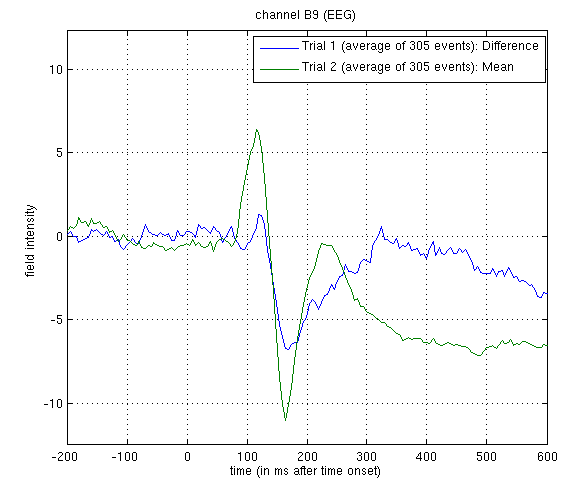
\includegraphics[width=100mm]{multimodal/figures/eeg_erp}
\caption{\em  Average (green) and differential (blue) ERPs for faces and scrambled faces at channel B9 in \texttt{wmaceMdspm8\_faces\_run1.mat}. \label{multimodal:fig:4}}
\end{center}
\end{figure}

The green line shows the average ERP evoked by faces and scrambled faces (at this occipitotemporal channel). A P1 and N1 are clearly seen. The blue line shows the differential ERP between faces and scrambled faces. The difference is small around the P1 latency, but large and negative around the N1 latency. The latter likely corresponds to the ``N170'' (Henson et al, 2003). We will try to localise the cortical sources of the P1 and N170 in Section~\ref{multimodal:eeg:3D}.

To see the topography of the differential ERP, click on Trial 1 again, press the ``topography'' icon button at the top of the window and scroll the latency from baseline to the end of the epoch. You should see a maximal difference around 180ms as in Figure~\ref{multimodal:fig:5} (possibly including a small delay of about 8ms for the CRT display to scan to the centre of the screen).

\begin{figure}
\begin{center}
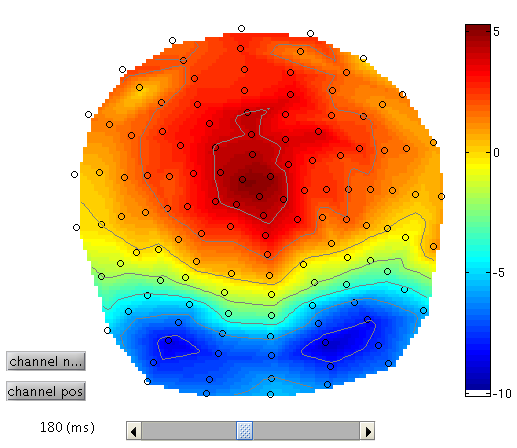
\includegraphics[width=100mm]{multimodal/figures/eeg_topo}
\caption{\em 2D topography for faces minus scrambled faces at 180ms. \label{multimodal:fig:5}}
\end{center}
\end{figure}

\subsection{3D SPMs (Sensor Maps over Time) \label{multimodal:eeg:3DSPM}}

A feature of SPM is the ability to use Random Field Theory to correct for multiple statistical comparisons across N-dimensional spaces. For example, a 2D space representing the scalp data can be constructed by flattening the sensor locations (using the 2D layout we created earlier) and interpolating between them to create an image of $M\times M$ pixels (when $M$ is user-specified, eg $M=32$). This would allow one to identify locations where, for example, the ERP amplitude in two conditions at a given timepoint differed reliably across subjects, having corrected for the multiple t-tests performed across pixels. That correction uses Random Field Theory, which takes into account the spatial correlation across pixels (i.e, that the tests are not independent). This kind of analysis is described earlier in the SPM manual, where a 1st-level design is used to create the images for a given weighting across timepoints of an ERP/ERF, and a 2nd-level design can then be used to test these images across subjects.

Here, we will consider a 3D example, where the third dimension is time, and test across trials within the single subject. We first create a 3D image for each trial of the two types, with dimensions $M\times M\times S$, where S=161 is the number of samples. We then take these images into an unpaired t-test across trials (in a 2nd-level model) to compare faces versus scrambled faces. We can then use classical SPM to identify locations in space and time in which a reliable difference occurs, correcting across the multiple comparisons entailed. This would be appropriate if, for example, we had no a priori knowledge where or when the difference between faces and scrambled faces would emerge\footnote{Note that the 2D location in sensor space for EEG will depend on the choice of montage.}.

Select the ``Convert to images'' option in the ``Other'' menu in the SPM main window, and select the \texttt{aceMdspm8\_faces\_run1.mat} file. You will then be prompted for ``output image dimensions'', for which you can accept the default of 32 (leading to a $32\times 32$ pixel space). It will then ask whether you want to interpolate or mask out bad channels, for which you select ``interpolate'' (though it will make no difference here because there are no bad channels).

This will take some time as it writes out an image for each trial (except rejected trials), in a new directory called \texttt{aceMdspm8\_faces\_run1}, which will itself contain two subdirectories, one for each trialtype. In each trialtype subdirectory there will be image and header files for each non-rejected trial of that type, e.g, \texttt{trial0002.\{hdr,img\}}. You can press ``Display: images'' to view one of these images - it will have dimensions $32\times 32\times 161$, with the origin set at [16 18.6 41] (where 41 samples is 0ms), as in Figure~\ref{multimodal:fig:6}.

\begin{figure}
\begin{center}
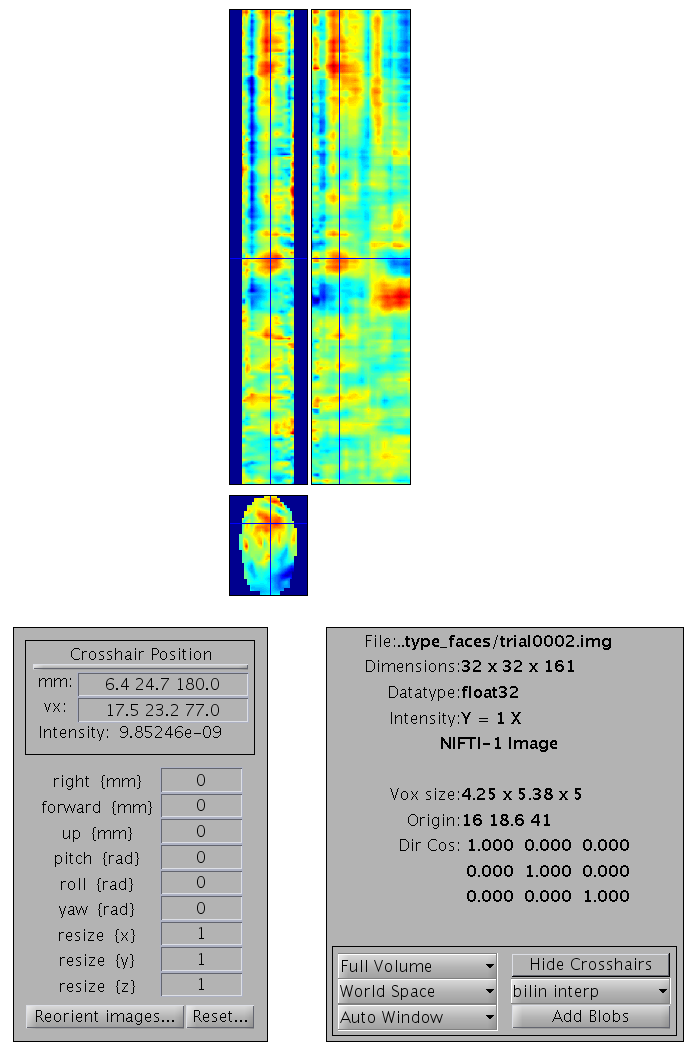
\includegraphics[width=120mm]{multimodal/figures/eeg_scalptime}
\caption{\em 3D image for trial 2 of \texttt{aceMdspm8\_faces\_run1.mat}. The bottom image is a 2D x-y space interpolated from the flattened electrode locations (at one point in time). The two top images are sections through x and y respectively, now expressed over time (vertical (z) dimension).\label{multimodal:fig:6}}
\end{center}
\end{figure}

To perform statistics on these images, first create a new directory, eg. \texttt{mkdir XYTstats}.

Then press the ``Specify 2nd level'' button, to produce the batch editor window again. Select the new \texttt{XYTstats} as the ``Directory'', and ``two-sample t-test'' (unpaired t-test) as the ``Design''. Then select the images for ``group 1 scans'' as all those in the subdirectory ``type\_faces'' (using right click, and ``select all'') and the images for ``group 2 scans'' as all those in the subdirectory ``type\_scrambled''. You might want to save this batch specification, but then press ``run''\footnote{Note that we can use the default ``nonsphericity'' selections, i.e, that the two trial-types may have different variances, but are uncorrelated.}.

This will produce the design matrix for a two-sample t-test.

Then press ``Estimate'', and when it has finished, press ``Results'' and define a new F-contrast as [1 -1]. Keep the default contrast options, but threshold at $p<.05$ FWE corrected for the whole search volume and select ``Scalp-Time'' for the ``Data Type''. Then press ``whole brain'', and the Graphics window should now look like that in Figure~\ref{multimodal:fig:7}.

This will reveal ``regions'' within the 2D sensor space and within the -200ms to 600ms epoch in which faces and scrambled faces differ reliably, having corrected for multiple F-tests across pixels and time. There are a number of such regions, but the largest has maxima at [-13 -78 180] and [21 -68 180], corresponding to left and right posterior sites at 180ms. The second largest has a maximum at [0 8 180], which is close to Cz. An F-test was used because the sign of the difference reflects the polarity of the ERP difference, which is not of primary interest (and depends on the choice of reference). Indeed, if you plot the contrast of interest from the cluster maxima, you will see that the difference is negative for the first posterior, cluster but positive for the second, central cluster. This is consistent with the polarity of the differences in Figure~\ref{multimodal:fig:5}\footnote{The former likely corresponds to the ``N170'', while the latter likely corresponds to the ``VPP'', which may be two signs of the same effect, though of course these effects depend on the choice of reference.}.

If one had more constrained a priori knowledge about where and when the N170 would appear, one could perform an SVC based on, for example, a box around posterior channels and between 150 and 200ms poststimulus. See \url{http://imaging.mrc-cbu.cam.ac.uk/meg/SensorSpm} for more details.

If you go to the global maximum, then press ``overlays'', ``sections'' and select the ``mask.img'' in the stats directory, you will get sections through the space-time image. A right click will reveal the current scalp location and time point. By moving the cursor around, you can see that the N170/VPP effects start to be significant (after whole-image correction) around 150ms (and may also notice a smaller but earlier effect around 100ms).

\begin{figure}
\begin{center}
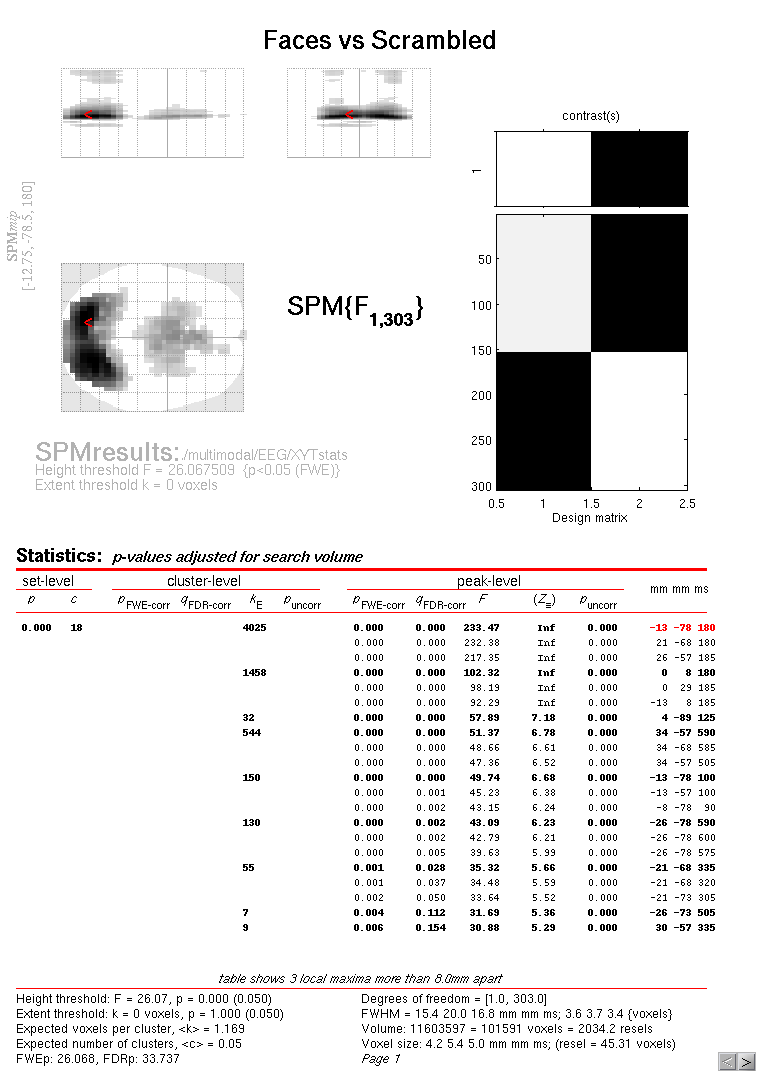
\includegraphics[width=120mm]{multimodal/figures/eeg_scalptime_results}
\caption{\em 3D sensor-time SPM{F} at $p<.05$ FWE corrected for the amplitude difference between face and scrambled face trials. The x, y coordinates refer to position in the 32x32 electrode plane (with units of mm); the z coordinate refers to peristimulus time in ms (to the nearest sampling of 5ms). \label{multimodal:fig:7}}
\end{center}
\end{figure}

\subsection{3D ``imaging'' reconstruction \label{multimodal:eeg:3D}}

Here we will demonstrate a distributed source reconstruction of the N170 differential evoked response between faces and scrambled faces, using a grey-matter mesh extracted from the subject's MRI, and the Multiple Sparse Priors (MSP) method in which multiple constraints on the solution can be imposed (Friston et al, 2008, Henson et al, 2009a).

Press the ``3D source reconstruction'' button, and press the ``load'' button at the top of the new window. Select the \verb!wmaceMdspm8_faces_run1.mat! file and type a label (eg "N170 MSP") for this analysis\footnote{Note that no new M/EEG files are created during the 3D reconstruction; rather, each step involves updating of the cell-array field \texttt{D.inv}, which will have one entry per analysis performed on that dataset (e.g, \texttt{D.inv\{1\}} in this case).}.

Press the ``MRI'' button, select the \texttt{smri.img} file within the \texttt{sMRI} sub-directory, and select ``normal'' for the cortical mesh.

The ``imaging'' option corresponds to a distributed source localisation, where current sources are estimated at a large number of fixed points (8196 for a ``normal'' mesh here) within a cortical mesh, rather than approximated by a small number of equivalent dipoles (the ECD option). The imaging  approach is better suited for group analyses and (probably) for later-occuring ERP components. The ECD approach may be better suited for very early sensory components (when only small parts of the brain are active), or for DCMs using a small number of regions (Kiebel et al, 2006).

The first time you use a particular structural image for 3D source reconstruction, it will take some time while the MRI is segmented (and normalisation parameters determined). This will create in the \texttt{sMRI} directory the files \texttt{y\_smri.nii} and \texttt{smri\_seg8.mat} for normalisation parameters and 4 GIfTI (\texttt{.gii}) files defining the cortical mesh, inner skull, outer skull and scalp surface.

When meshing has finished, the cortex (blue), inner skull (red), outer skull (orange) and scalp (pink) meshes will be shown in the Graphics window with slices from the sMRI image, as shown in Figure~\ref{multimodal:fig:3}. This makes it possible to visually verify that the meshes fit the original image well. The field \texttt{D.inv\{1\}}.mesh field will be updated in \matlab\ . Press ``save'' in top right of window to update the corresponding \texttt{mat} file on disk.

\begin{figure}
\begin{center}
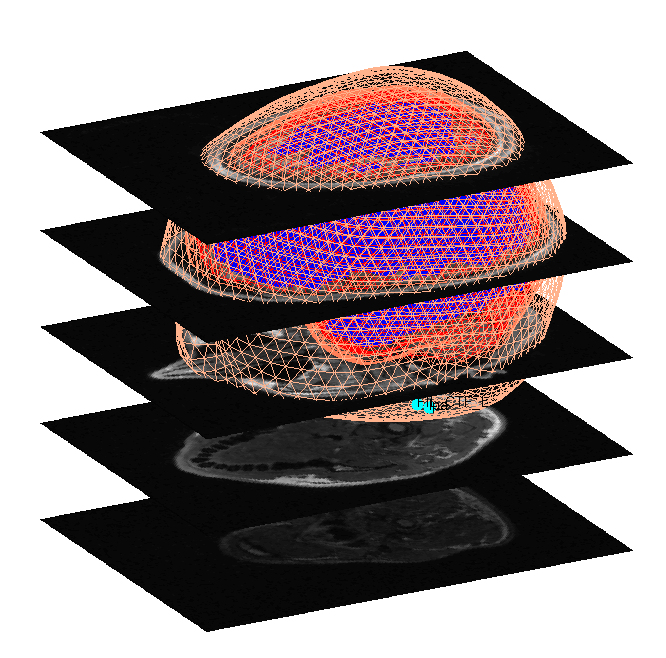
\includegraphics[width=90mm]{multimodal/figures/eeg_meshing}
\caption{\em Cortex (blue), inner skull (red), outer skull (orange) and scalp (pink) meshes with transverse slices of the subject's MRI. \label{multimodal:fig:3}}
\end{center}
\end{figure}

Both the cortical mesh and the skull and scalp meshes are not created directly from the segmented MRI, but rather are determined from template meshes in MNI space via inverse spatial normalisation (Mattout et al, 2007).

Press the ``Co-register'' button. You will first be asked to select at least 3 fiducials from a list of points in the EEG dataset (from Polhemus file): by default, SPM has already highlighted what it thinks are the fiducials, i.e, points labelled ``nas'' (nasion), ``lpa'' (left preauricular) and ``rpa'' (right preauricular). So just press ``ok''.

You will then be asked for each of the 3 fiducial points to specify its location on the MRI images. This can be done by selecting a corresponding point from a hard-coded list (``select''). These points are inverse transformed for each individual image using the same deformation field that is used to create the meshes. The other two options are typing the MNI coordinates for each point (``type'') or clicking on the corresponding point in the image (``click''). Here, we will type coordinates based on where the experimenter defined the fiducials on the \texttt{smri.img}. These coordinates can be found in the \texttt{smri\_fid.txt} file also provided. So press ``type'' and for ``nas'', enter [0 91 -28]; for ``lpa'' press ``type'' and enter [-72 4 -59]; for ``rpa'' press ``type'' and enter [71 -6 -62]. Finally, answer ``yes'' to ``Use headshape points?''.

This stage coregisters the EEG sensor positions with the structural MRI and cortical mesh, via an approximate matching of the fiducials in the two spaces, followed by a more accurate surface-matching routine that fits the head-shape function (measured by Polhemus) to the scalp that was created in the previous meshing stage via segmentation of the MRI. When coregistration has finished, the field D.inv\{1\}.datareg will be updated in \matlab\ . Press ``save'' in top right of window to update the corresponding mat file on disk. With the \matlab\ Rotation tool on (from the ``Tools'' tab in the SPM Graphics window, if not already on), right click near the top image and select ``Go to Y-Z'' view (if the image has disappeared press the display button underneath co-register). Finally, a figure like that in Figure~\ref{multimodal:fig:8} will also be produced, which you can rotate with the mouse (using the Rotate3D \matlab\ Menu option) to check all sensors.

Note that for these data, the coregistration is not optimal, with several EEG electrodes appearing inside the scalp.  This may be inaccurate Polhemus recording of the headshape or inaccurate surface matching for the scalp mesh, or ``slippage'' of headpoints across the top of the scalp (which might be reduced in future by digitising features like the nose and ears, and including them in the scalp mesh). In the meantime, if this happens in your data, you can stick with fiducials if you are confident that you can localise them reliably and accurately. This is not actually a problem for the BEM calculated below, however, because the electrodes are re-projected to the scalp surface (as a precaution).

\begin{figure}
\begin{center}
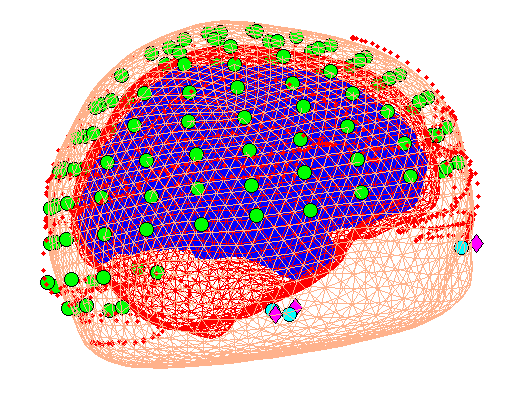
\includegraphics[width=70mm]{multimodal/figures/eeg_coreg.png}
\caption{\em  Graphical output of Co-registration of EEG data, showing (upper panel) cortex (blue), inner skull (red) and scalp (black) meshes, electrode locations (green), MRI/Polhemus fiducials (cyan/magneta), and headshape (red dots).\label{multimodal:fig:8}}
\end{center}
\end{figure}

Press ``Forward Model'', and select ``EEG BEM''. The first time you do this, there will be a lengthy computation and a large file \texttt{smri\_EEG\_BEM.mat} will be saved in the \texttt{sMRI} directory containing the parameters of the boundary element model (BEM). In the Graphics window the BEM meshes will be displayed with the EEG sensors marked with green asterisks as shown in Figure~\ref{multimodal:fig:2}. This display is the final quality control before the model is used for lead field computation.

\begin{figure}
\begin{center}
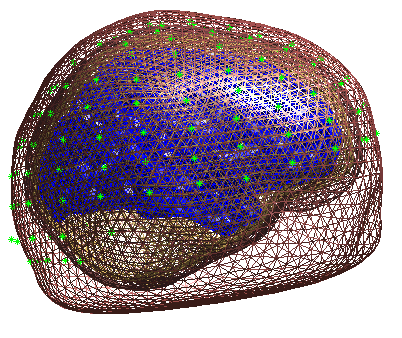
\includegraphics[width=70mm]{multimodal/figures/eeg_forward.png}
\caption{\em BEM meshes with the EEG sensors marked as asterisks.\label{multimodal:fig:2}}
\end{center}
\end{figure}

Press ``Invert'', select ``Imaging'' (i.e, a distributed solution rather than DCM; Kiebel et al (2006)), select ``yes'' to include all conditions (i.e, both the differential and common effects of faces and scrambled faces) and then ``Standard'' to use the default settings.

By default the MSP method will be used. MSP stands for ``Multiple Sparse Priors'' (Friston et al. 2008a), and has been shown to be superior to standard minimum norm (the alternative IID option) or a maximal smoothness solution (like LORETA; the COH option) - see Henson et al (2009a). Note that by default, MSP uses a ``Greedy Search'' (GS) (Friston et al, 2008b), though the standard ReML (as used in Henson et al, 2007) can also be selected (this uses Automatic Relevance Determination - ARD).

The ``Standard'' option uses default values for the MSP approach (to customise some of these parameters, press ``Custom'' instead).

At the first stage of the inversion lead fields will be computed for all the mesh vertices and saved in the file \texttt{SPMgainmatrix\_wmaceMdspm8\_faces\_run1\_1.mat}. Then the actual MSP algorithm will run and the summary of the solution will be displayed in the Graphics window.

Press ``save'' to save the results. You can now explore the results via the 3D reconstruction window. If you type 180 into the box in the bottom right (corresponding to the time in ms) and press ``mip'', you should see an output similar to Figure~\ref{multimodal:fig:9}. This fit explains approx 98\% of the data.

Note the hot-spots in the posterior and mid-lateral ventral temporal lobe. The timecourses come from the peak voxel. The red curve shows the condition currently being shown (corresponding to the ``Condition 1'' toggle bar in the reconstruction window); the grey line(s) will show all other conditions. ``Condition 1'' is the differential evoked responses for faces vs scrambled; if you press the ``condition 1'' toggle, it will change to ``Condition 2'' (average evoked response for faces and scrambled faces), then press ``mip'' again and the display will update (note the colours of the lines have now reversed from before, with red now corresponding to average ERP). For the average effect, change the time to 100ms, and note mainly posterior occipital activation (though also some strong medial sources, the biological validity of which is unclear).

If you toggle back to ``Condition 1'' and press ``movie'', you will see changes in the source strengths for the differential response over peristimulus time (from the limits 0 to 300ms currently chosen by default).
If you press ``render'' you can get a very neat graphical interface to explore the data (the buttons are fairly self-explanatory). 

You can also explore other inversion options, such as COH and IID (available for the ``custom'' inversion), which you will notice give more superficial solutions (a known problem with standard minimum norm approaches). To do this quickly (without repeating the MRI segmentation, coregistration and forward modelling), press the ``new'' button in the reconstruction window, which by default will copy these parts from the previous reconstruction.

In this final section we will concentrate on how to prepare source data for subsequent statistical analysis (eg with data from a group of subjects).

\begin{figure}
\begin{center}
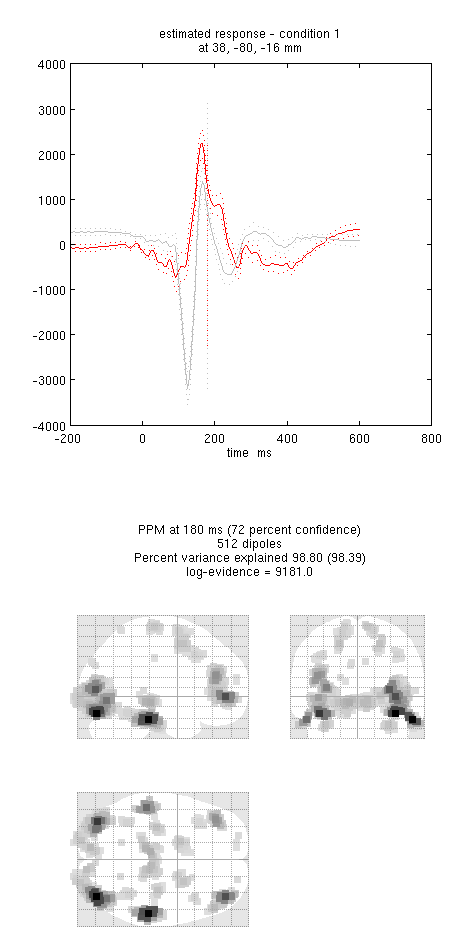
\includegraphics[width=90mm]{multimodal/figures/eeg_msp.png}
\caption{\em Graphical output of an MSP estimation of the differential ERP between faces and scrambled faces at 180ms. \label{multimodal:fig:9}}
\end{center}
\end{figure}

Press the ``Window'' button in the reconstruction window, enter ``150 200'' as the timewindow of interest and keep ``0'' as the frequency band of interest (0 means all frequencies). The Graphics window will then show the mean activity for this time/frequency contrast (top plot) and the contrast itself (bottom plot; note additional use of a Hanning window).

Then press ``Image'', ``12'' for the smoothing kernel, and SPM will write 3D NIfTI images corresponding to the above contrast for each condition:
\begin{verbatim}
    w_wmaceMdspm8_faces_run1_1_1.nii
    w_wmaceMdspm8_faces_run1_1_2.nii
    sw_wmaceMdspm8_faces_run1_1_1.nii
    sw_wmaceMdspm8_faces_run1_1_2.nii
\end{verbatim}
Note that the first two images are unsmoothed (but normalised); the latter two are the result of smoothing the former two by a 12mm isotropic Gaussian kernel. The last number in the file name refers to the condition number; the penultimate number refers to the reconstruction number (i.e. the number in red in the reconstruction window, i.e, \texttt{D.val}, here 1). The reconstruction number will increase if you create a new inversion by pressing ``new''.

The smoothed results for Condition 1 (i.e, the differential evoked response for faces vs scrambled faces) will also be displayed in the Graphics window, see Figure~\ref{multimodal:fig:eegrecon}, together with the normalised structural. Note that the solution image is in MNI (normalised) space, because the use of a canonical mesh provides us with a mapping between the cortex mesh in native space and the corresponding MNI space.

You can also of course view the image with the normal SPM ``Display:image'' option (just the functional image with no structural will be shown), and locate the coordinates of the ``hotspots'' in MNI space. Note that these images contain RMS (unsigned) source estimates (see Henson et al, 2007).
Given that one has data from multiple subjects, one can create a NIFTI file for each. Group statistical analysis can the be implemented with eg. second level t-tests as described earlier in the chapter.


\begin{figure}[h!t]
\begin{center}
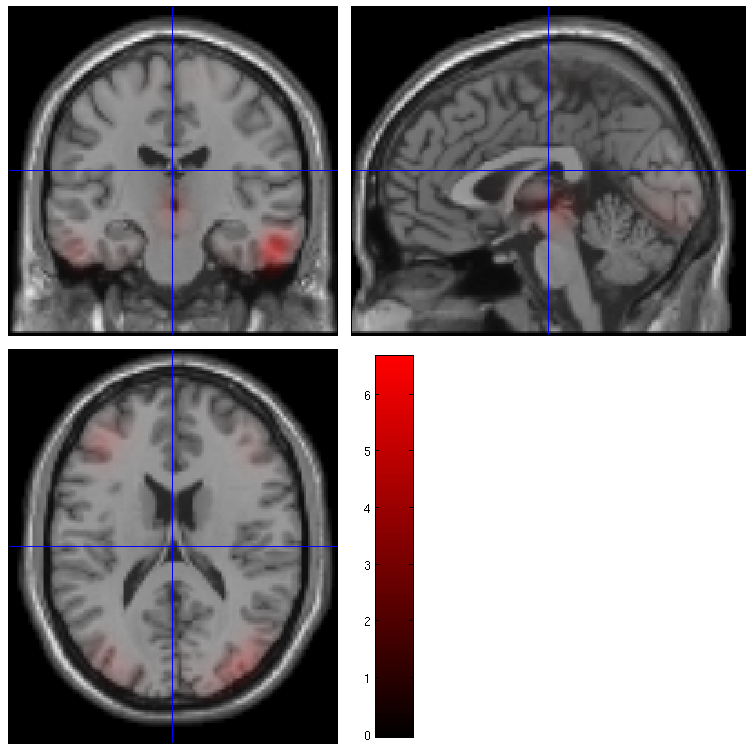
\includegraphics[width=90mm]{multimodal/figures/eeg_recon.png}
\caption{\em 3D reconstruction saved as a smoothed NIfTI image of the differential evoked response for faces vs scrambled faces around the N170. \label{multimodal:fig:eegrecon}}
\end{center}
\end{figure}


\section{MEG analysis \label{multimodal:data:meg}}

\subsection{Preprocessing the MEG data\label{multimodal:data:meg:preproc}}

First change directory to the MEG subdirectory (either in \matlab\, or via the ``CD'' option in the SPM ``Utils'' menu)

\subsection{Adjust trigger latency}

For the EEG data, the faces were displayed directly via a CRT monitor. For the MEG data on the other hand, the faces were displayed inside the MSR via a projector. This projector produces a delay of 1.5 screen refreshes, which at 60Hz, is 25ms. This means that the subject actually saw the stimuli 25ms after the trigger was sent to the MEG acquisition machine. To correct for this visual delay, we will illustrate how to manipulate ``trial'' structures\footnote{Alternatively, you could correct by 1 refresh, to match the delay in the EEG data.}. First, we need to read in the triggers from the MEG data (unlike the EEG dataset, the MEG dataset contains information about trial type so we can define the correct condition labels already at this stage). To do this, type the following in the \matlab\ window:

\begin{verbatim}
    [trl, conditionlabels, S] = spm_eeg_definetrial;
\end{verbatim}

and follow these steps:
\begin{itemize}
 \item Select the \texttt{SPM\_CTF\_MEG\_example\_faces1\_3D.ds/SPM\_CTF\_MEG\_example\_faces1\_3D.meg4} file.
 \item Enter \texttt{-200} for ``Start of trial in PST [ms]'' and \texttt{600} to ``End of trial in PST [ms]''.
 \item Enter 2 for ``How many conditions?''.
 \begin{itemize}
  \item Enter ``\texttt{faces}'' for ``Label of condition 1''. A dialog with a list of events will come up and Select the event with type \texttt{UPPT001\_up} and Value 1.
  \item Enter ``\texttt{scrambled}'' for ``Label of condition 2''. Select the even with type \texttt{UPPT001\_up} and Value 2.
 \end{itemize}
 \item Answer ``no'' to the question about reviewing trials.
 \item Answer ``yes'' to the prompt to save the trial definition.
 \item Enter a filename like \texttt{trials\_run1.mat} and save in the MEG directory.
\end{itemize}

Then type \texttt{load trials\_run1.mat} in \matlab\, to see the contents of the file you just saved. It contains two variables, \texttt{trl} and \texttt{conditionlabels}. The \texttt{trl} variable contains as many rows as triggers were found (across all conditions) and three columns: the initial sample of the epoch, the final sample of the epoch and the offset in samples corresponding to a peristimulus time of 0. The sampling rate for the MEG data was 480Hz (as can be found in the \texttt{S.fsample} field of the structure \texttt{S} returned by the \texttt{spm\_eeg\_definetrial} call above). Thus the figure of -96 samples in the third column corresponds to the 200ms baseline period that you specified. Now we need to shift the initial and final samples of the epochs by 25ms. You can do this by typing:

\begin{verbatim}
    trl(:,1:2) = trl(:,1:2) + round(25*S.fsample/1000);
    save trials_run1 trl conditionlabels
\end{verbatim}

The new trial definition is thus resaved, and we can use this file when next converting the data.

\subsection{Convert}

Press the \textsc{Convert} button, and in the file selection window again select the \texttt{SPM\_CTF\_MEG\_example\_\-faces1\_3D.ds} subdirectory and the \texttt{\hyphenchar\font45\relax SPM\_CTF\_MEG\_example\_faces1\_3D.meg4} file. At the prompt ``Define settings?'' select ``yes''. Here we will use the option to define more precisely the part of data that should be read during conversion. Answer ``trials'' to ``How to read?'', and ``file'' to ``Where to look for trials?''. Then in the file selector window, select the new \texttt{trials\_run1.mat} file. Press ``no'' to ``Read across trials?'' and select ``meg'' for ``What channels?''. Press ``no'' to avoid saving the channel selection. Press ``Enter'' to accept the default suggestion for the name of the output dataset. Two files will be generated \texttt{espm8\_SPM\_CTF\_MEG\_example\_faces1\_3D.mat} and \texttt{espm8\_SPM\_CTF\_MEG\_example\_faces1\_3D.dat}. After the conversion is complete the data file will be automatically opened in the SPM8 reviewing tool. If you click on the ``MEG'' tab you will see the MEG data which is already epoched. By pressing the ``intensity rescaling'' button (with arrows pointing up and down) several times you will start seeing MEG activity.

\subsection{Baseline correction}

We need to perform baseline correction as it is not done automatically during conversion. This will prevent excessive edge artefacts from appearing after subsequent filtering and downsampling. Select \textsc{Baseline correction} from the ``Other'' drop-down menu and select the \texttt{espm8\_SPM\_CTF\_MEG\_example\_faces1\_3D.mat} file. Enter $[-200\: 0]$ for ``Start and stop of baseline [ms]''. The progress bar will appear and the resulting data will be saved to dataset \texttt{bespm8\_SPM\_\-CTF\_\-MEG\_\-example\_faces1\_3D.\{mat,dat\}}.

\subsection{Downsample}

Select \textsc{Downsample} from the ``Other'' drop-down menu and select the \texttt{bespm8\_SPM\_CTF\_\-MEG\_\-example\_\-faces1\_3D.mat} file. Choose a new sampling rate of 200 (Hz). The progress bar will appear and the resulting data will be saved to dataset \texttt{dbespm8\_SPM\_CTF\_MEG\_example\_faces1\_3D.\{mat,dat\}}.

\subsection{Batch preprocessing}

Here we will preprocess the second half of the MEG data using using the SPM8 batch facility to demonstrate this third (after interactive GUI and Matlab script) possibility. First though, we have to correct the visual onset latency for the second run, repeating the above steps that you did for the first run:

\begin{verbatim}
    [trl, conditionlabels, S] = spm_eeg_definetrial;
\end{verbatim}

and select the \texttt{SPM\_CTF\_MEG\_example\_faces2\_3D.ds} subdirectory and the \texttt{SPM\_\-CTF\_\-MEG\_\-example\_\-faces2\_3D.meg4} file. Then enter \texttt{-200} for ``Start of trial in PST [ms]'' and \texttt{600} to ``End of trial in PST [ms]''. Enter \texttt{2} for ``How many conditions?''. Enter ``\texttt{faces}'' for ``Label of condition 1''. A dialog with a list of events will come up. Select the event with type ``\texttt{UPPT001\_up}'' and Value 1. Enter \texttt{scrambled} for ``Label of condition 2''. Select the event with type ``\texttt{UPPT001\_up}'' and Value 2. Answer ``no'' to the question about reviewing trials, but ``yes'' to the prompt to save the trial definition. Enter a filename like \texttt{trials\_run2.mat} and save in the MEG directory. Then type:

\begin{verbatim}
    load trials_run2
    trl(:,1:2) = trl(:,1:2)+round(25*S.fsample/1000);
    save trials_run2 trl conditionlabels
\end{verbatim}

Now press the \textsc{Batch} button (lower right corner of the SPM8 menu window). The batch tool window will appear. We will define exactly the same settings as we have just done using the interactive GUI. From the ``SPM'' menu, ``M/EEG'' submenu select ``M/EEG Conversion''. Click on ``File name'' and select the \texttt{SPM\_CTF\_MEG\_example\_faces2\_3D.meg4} file from \texttt{SPM\_CTF\_\-MEG\_\-example\_\-faces2\_3D.ds} subdirectory. Click on ``Reading mode'' and switch to ``Epoched''. Click on ``Epoched'' and choose ``Trial file'', double-click on the new ``Trial file'' branch and then select the \texttt{trials\_run2.mat} file.  Then click on ``Channel selection'' and select MEG from the menu below. Finally enter \texttt{espm8\_SPM\_CTF\_MEG\_example\_faces2\_3D} for ``Output filename'' to be consistent with the file preprocessed interactively.

Now select ``M/EEG Baseline correction'' from the ``SPM'' menu, ``M/EEG'' submenu. Another line will appear in the Module list on the left. Click on it. The baseline correction configuration branch will appear. Select ``File name'' with a single click. The file that we need to downsample has not been generated yet but we can use the ``Dependency'' button. A dialog will appear with a list of previous steps (in this case just the conversion) and we can set the output of one of these steps as the input to the present step. Now just enter enter $-200\: 0$ for ``Baseline''. Similarly we can now add ``M/EEG Downsampling'' to the module list, define the output of baseline correction step for ``File name'' and 200 for the ``New sampling rate''. This completes our batch. We can now save it for future use (e.g, as \texttt{batch\_meg\_preprocess} and run it by pressing the green ``Run'' button. This will generate all the intermediate datasets and finally \texttt{dbespm8\_SPM\_CTF\_MEG\_example\_faces2\_3D.\{mat,dat\}}.

\subsection{Merge}

We will now merge the two epoched files we have generated until now and continue working on the merged file. Select the \textsc{Merge} command from the ``Other'' drop-down menu. In the selection window that comes up click on \texttt{dbespm8\_SPM\_CTF\_MEG\_example\_faces1\_3D.mat} and \texttt{dbespm8\_SPM\_CTF\_MEG\_example\_faces2\_3D.mat}. Press ``done''. Answer ``Leave as they are'' to ``What to do with condition labels?''. A new dataset will be generated called \texttt{cdbespm8\_SPM\_CTF\_\-MEG\_\-example\_\-faces1\_\-3D.\{mat,dat\}}.

\subsection{Reading and preprocessing data using Fieldtrip}
Yet another even more flexible way to pre-process data in SPM8 is to use the Fieldtrip toolbox (\url{http://www.ru.nl/neuroimaging/fieldtrip/}) that is distributed with SPM. All the pre-processing steps we have done until now can also be done in Fieldtrip and the result can then be converted to SPM8 dataset. An example script for doing so can be found in the 
\texttt{man$\backslash$example\_scripts$\backslash$spm\_ft\_multimodal\_preprocessing.m}. The script will generate a merged dataset and save it under the name \texttt{ft\_SPM\_CTF\_\-MEG\_\-example\_\-faces1\_\-3D.\{mat,dat\}}. The rest of the analysis can then be done as below. This option is more suitable for expert users well familiar with Matlab. Note that in the script \texttt{ft\_} prefix is added to the names of all Fieldtrip functions. This is a way specific to SPM8 to call the functions from Fieldtrip version included in SPM distribution and located under \texttt{external$\backslash$fieldtrip}.

\subsection{Prepare}

In this section we will add the separately measured headshape points to our merged dataset. This is useful when one wants to improve the coregistration using head shape measured outside the MEG. Also in some cases the anatomical landmarks detectable on the MRI scan and actual locations of MEG locator coils do not coincide and need to be measured in one common coordinate system by an external digitizer (though this is not the case here). First lets examine the contents of the headshape file. If you load it into \matlab\ workspace (type \texttt{load headshape.mat}), you will see that it contains one \matlab\ structure called \texttt{shape} with the following fields:
\begin{itemize}
\item \texttt{.unit} - units of the measurement (optional)
\item \texttt{.pnt} - Nx3 matrix of headshape points
\item \texttt{.fid} - substruct with the fields .pnt - Kx3 matrix of points and .label -Kx1 cell array of point labels.
\end{itemize}

The difference between \texttt{shape.pnt} and \texttt{shape.fid.pnt} is that the former contains unnamed points (such as continuous headshape measurement) whereas the latter contains labeled points (such as fiducials). Note that this Polhemus space (which will define the ``head space'') has the X and Y axes switched relative to MNI space.

Now select \textsc{Prepare} from the ``Other'' menu and in the file selection window select \texttt{cdbespm8\_\-SPM\_\-CTF\_\-MEG\_\-example\_\-faces1\_3D.mat}. A menu will appear at the top of SPM interactive window (bottom left window). In the ``Sensors'' submenu choose ``Load MEG Fiducials/Headshape''. In the file selection window choose the \texttt{headshape.mat} file and save the dataset with \texttt{File/Save}.

If you do not have a separately measured headshape and are planning to use the original MEG fiducials for coregistration, this step is not necessary. As an exercise, you can skip it for the tutorial dataset and later do the coregistration without the headshape and see if it affects the results.

\subsection{Basic ERFs} 

Press the \textsc{Averaging} button and select the \texttt{cdbespm8\_SPM\_CTF\_MEG\_example\_faces1\_3D.mat} file. Answer ``yes'' to ``Use robust averaging?''. You can either save the weights if you want to examine them or not save if you want the averaging to work faster since the weights dataset that needs to be written is quite large. Answer ``no'' to ``weight by condition'' and accept the default ``Offset of the weighting function''. A new dataset will be created in the MEG directory called \texttt{mcdbespm8\_SPM\_CTF\_MEG\_example\_faces1\_3D.\{mat,dat\}} (``m'' for ``mean'').

As before, you can display these data by ``Display: M/EEG'' and selecting the \texttt{mcdbespm8\_\-SPM\_\-CTF\_\-MEG\_\-example\_\-faces1\_3D.mat}. In the MEG tag with the scalp radio button selected, hold the Shift key and select trial-type 2 with the mouse in the bottom right of the window to see both conditions superimposed (as Figure~\ref{multimodal:fig:10}).

\begin{figure}
\begin{center}
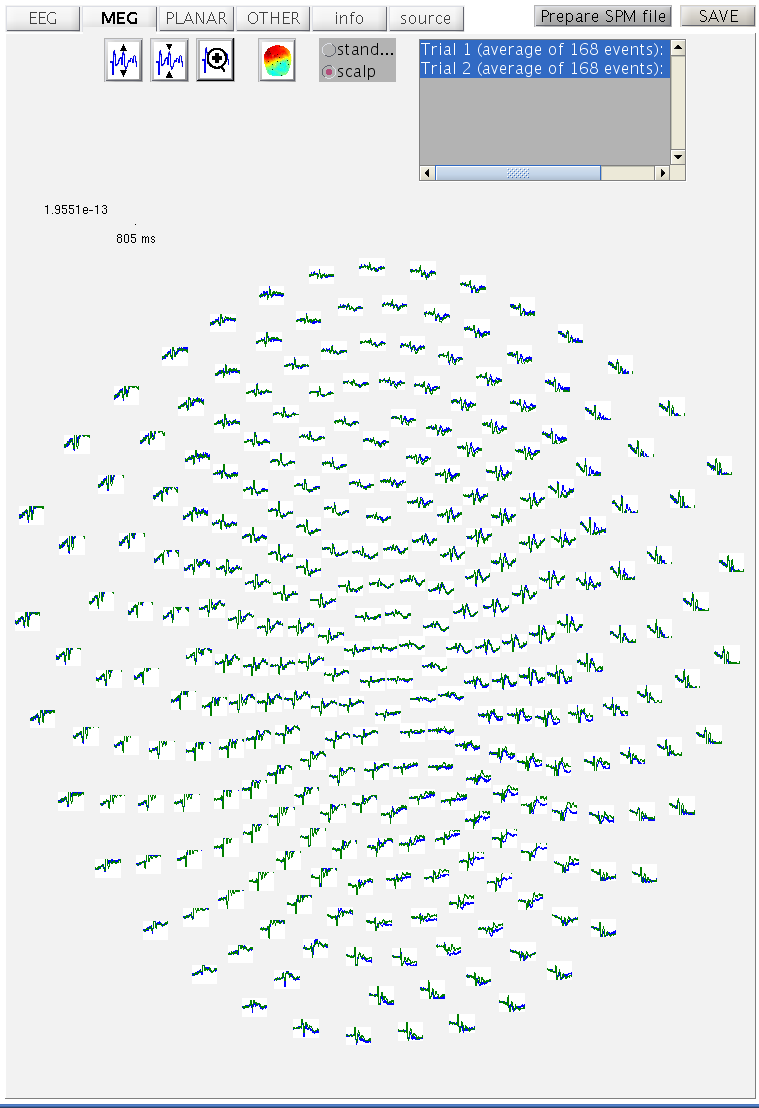
\includegraphics[width=100mm]{multimodal/figures/meg_scalp_erf}
\caption{\em SPM Display window for mean, smoothed ERF (\texttt{mcdbespm8\_\-SPM\_\-CTF\_\-MEG\_\-example\_\-faces1\_\-3D.mat}) for all 275 MEG channels. \label{multimodal:fig:10}}
\end{center}
\end{figure}

Select ``Contrast'' from the ``Other'' pulldown menu on the SPM window. This function creates linear contrasts of ERPs/ERFs. Select the \texttt{mcdbespm8\_SPM\_CTF\_MEG\_example\_faces1\_3D.mat} file, enter $[1\: -1]$ as the first contrast and label it ``\texttt{Difference}'', answer ``yes'' to ``Add another'',  enter $[1/2\: 1/2]$ as the second contrast and label it ``\texttt{Mean}''. Press ``no'' to the question ``Add another'' and not to ``weight by num replications''. This will create new file \texttt{wmcdbespm8\_\-SPM\_\-CTF\_\-MEG\_\-example\_\-faces1\_\-3D.mat}, in which the first trial-type is now the differential ERF between faces and scrambled faces, and the second trial-type is the average ERF for faces and scambled faces.

To see the topography of the differential ERF, select ``Display: M/EEG'', MEG tab and click on Trial 1, press the ``topography'' button at the top of the window and scroll to 180ms for the latency to produce Figure~\ref{multimodal:fig:12}.

You can move the slider left and right to see the development of the M170 over time.

\begin{figure}
\begin{center}
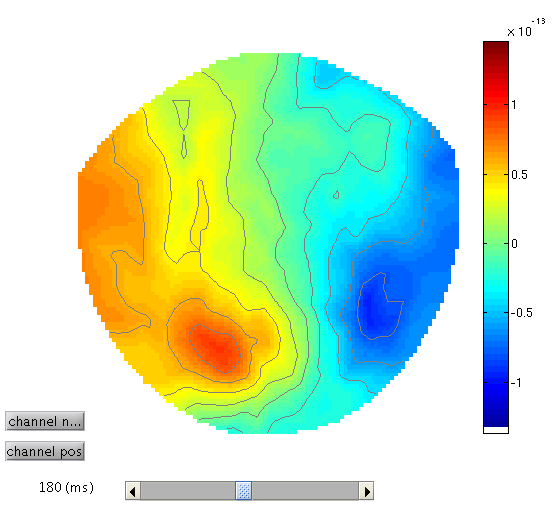
\includegraphics[width=100mm]{multimodal/figures/meg_topo180}
\caption{\em 2D topography of the ERF of faces minus scrambled faces at 180ms. \label{multimodal:fig:12}}
\end{center}
\end{figure}

\subsection{Time-Frequency Analysis}

SPM uses Morlet wavelets to perform time-frequency analyses.

Select the \textsc{time-frequency} option under the ``Other'' pull-down menu, and select the \texttt{cdbespm8\_\-SPM\_\-CTF\_\-MEG\_\-example\_\-faces1\_\-3D.mat} file. SPM will then prompt you for the frequencies you wish to analyse, for which you can type [5:40] (Hz). Change the default Morlet wavelet order (N) from 7 to 5. This factor effectively trades off frequency vs time resolution, with a lower order giving higher temporal resolution. You will then be prompted to select channels from a list. Select ``MLT34'' and press ``OK''\footnote{You can of course obtain time-frequency plots for every channel, but it will take much longer (and result in a large file).}. Answer ``yes'' to ``Compute phase?''.

This will produce two new datasets, \texttt{tf1\_\-cdbespm8\_\-SPM\_\-CTF\_\-MEG\_\-example\_\-faces1\_3D.\{mat,dat\}} and  \texttt{tf2\_\-cdbespm8\_\-SPM\_\-CTF\_\-MEG\_\-example\_\-faces1\_\-3D.\{mat,dat\}}. The former contains the power at each frequency, time and channel; the latter contains the corresponding phase angles.

Here we will not baseline correc the time-frequency data because for frequencies as low as 5Hz, one would need a longer pre-stimulus baseline, to avoid edge-effects\footnote{For example, for 5Hz, one would need at least N/2 x 1000ms/5, where N is the order of the Morlet wavelets (i.e, number of cycles per Gaussian window), e.g, 600ms for a 6th-order wavelet.}. Later, we will compare two trial-types directly, and hence any pre-stimulus differences will become apparent. 

Press the \textsc{Averaging} button and select the \texttt{tf1\_\-cdbespm8\_\-SPM\_\-CTF\_\-MEG\_\-example\_\-faces1\_\-3D.mat} file. You can use straight (or robust if you prefer) averaging to compute the average time-frequency representation. A new file will be created in the MEG directory called \texttt{mtf1\_cdbespm8\_\-SPM\_\-CTF\_\-MEG\_\-example\_\-faces1\_\-3D.\{mat,dat\}}. Note that you can use the reviewing tool to review the time-frequency datasets.

This contains the power spectrum averaged over all trials, and will include both ``evoked'' and ``induced'' power. Induced power is (high-frequency) power that is not phase-locked to the stimulus onset, which is therefore removed when averaging the amplitude of responses across trials (i.e, would be absent from a time-frequency analysis of the \texttt{mcdbespm8\_SPM\_\-CTF\_\-MEG\_\-example\_\-faces1\_\-3D.mat} file).

The power spectra for each trial-type can be displayed using the usual Display button and selecting the \texttt{mtf1\_\-cdbespm8\_\-SPM\_\-CTF\_\-MEG\_\-example\_\-faces1\_3D.mat} file. This will produce a plot of power as a function of frequency (y-axis) and time (x-axis) for Channel MLT34. If you use the ``trial'' slider to switch between trial(types) 1 and 2, you will see the greater power around 150ms and 10Hz for faces than scrambled faces (click on the magnifying glass icon and on the single channel to get scales for the axes, as in Figure~\ref{multimodal:fig:13}). This corresponds to the M170 again.

\begin{figure}
\begin{center}
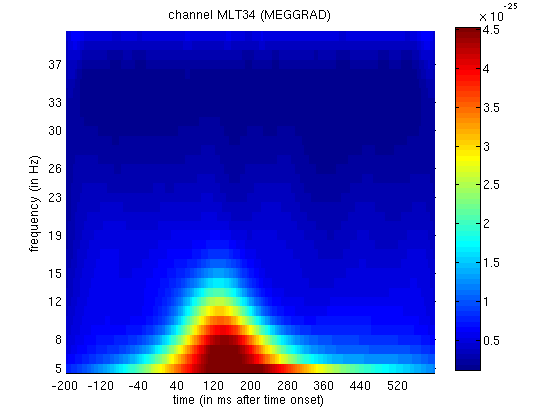
\includegraphics[width=60mm]{multimodal/figures/meg_pow_faces}
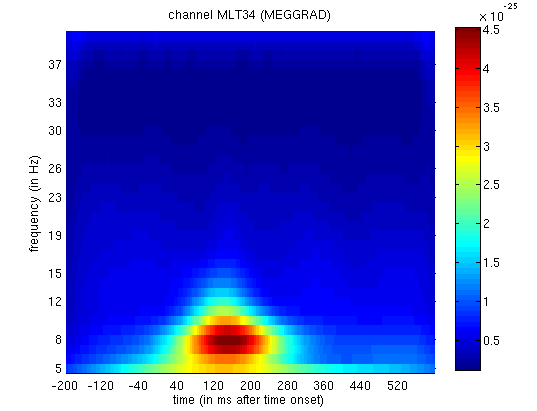
\includegraphics[width=60mm]{multimodal/figures/meg_pow_scrambled}
\caption{\em  Total power spectra for faces (left) and scrambled faces (right) for channel MLT34\label{multimodal:fig:13}}
\end{center}
\end{figure}

We can also look at evidence of phase-locking of ongoing oscillatory activity by averaging the phase angle information. We compute the vector mean (by converting the angles to vectors in Argand space), which yelds  complex numbers. We can generate two kinds of images from these numbers. The first is an image of the angles, which shows the mean phase of the oscillation (relative to the trial onset) at each time point. The second is an image of the absolute values (also called ``Phase-Locking Value'', PLV) which lie between 0 for no phase-locking across trials and 1 for perfect phase-locking.

Press the \textsc{Averaging} button and select the \texttt{tf2\_\-cdbespm8\_\-SPM\_\-CTF\_\-MEG\_\-example\_\-faces1\_\-3D.mat} file. This time you will be prompted for either ``angle'' or ``abs(PLV)'' average, for which you should select ``abs(PLV)''. The \matlab\ window will echo:

\begin{verbatim}
  mtf2_cdbespm8_SPM_CTF_MEG_example_faces1_3D.mat: Number of replications per contrast:
  average faces: 168 trials, average scrambled: 168 trials
\end{verbatim}

and a new file will be created in the MEG directory called \texttt{mtf2\_\-cdbespm8\_\-SPM\_\-CTF\_\-MEG\_\-example\_\-faces1\_\-3D.mat}.

If you now display the file \texttt{mtf2\_\-cdbespm8\_\-SPM\_\-CTF\_\-MEG\_\-example\_\-faces1\_\-3D.mat} file, you will see PLV as a function of frequency (y-axis) and time (x-axis) for Channel MLT34. Again, if you use the ``trial'' slider to switch between trial(types) 1 and 2, you will see greater phase-locking around for faces than scrambled faces at lower frequencies, as in Figure~\ref{multimodal:fig:14}. Together with the above power analysis, these data suggest that the M170 includes an increase both in power and in phase-locking of ongoing oscillatory activity in the alpha range (Henson et al, 2005b).

\begin{figure}
\begin{center}
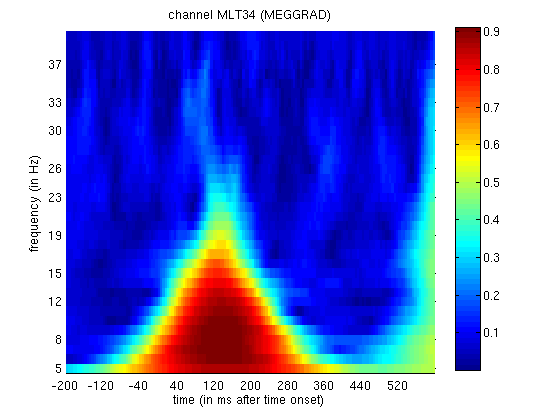
\includegraphics[width=60mm]{multimodal/figures/meg_plv_faces}
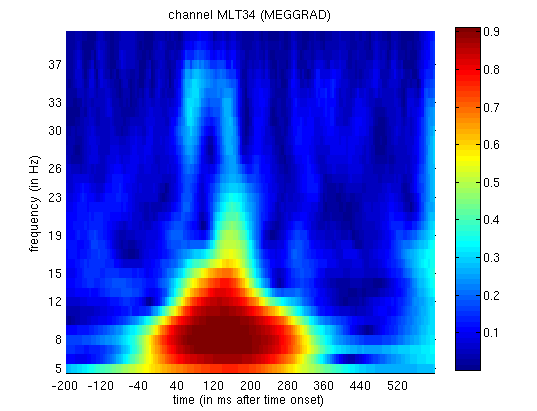
\includegraphics[width=60mm]{multimodal/figures/meg_plv_scrambled}
\caption{\em Phase-Locking Values for faces (left) and scrambled faces (right) for channel MLT34 \label{multimodal:fig:14}}
\end{center}
\end{figure}

\subsection{2D Time-Frequency SPMs}

Analogous to Section~\ref{multimodal:eeg:3DSPM}, we can also use Random Field Theory to correct for multiple statistical comparisons across the 2-dimensional time-frequency space.

Select \textsc{Convert to images} in the ``Other'' pulldown menu, and select the \texttt{tf1\_cdbespm8\_\-SPM\_\-CTF\_\-MEG\_\-example\_\-faces1\_\-3D.mat} file. Usually you would be asked whether you want to average over channels or frequencies. In this case there is only one channel in this dataset, so the ``channels'' option will be selected automatically.

This will create 2D time-frequency images for each trial of the two types with dimensions $36\times 161\times 1$, as for the example shown in Figure~\ref{multimodal:fig:15}. These images can be found in the subdirectories \texttt{1ROI\_TF\_\-trialtype\_\-faces} and \texttt{1ROI\_TF\_\-trialtype\_\-scrambled} of the new directory created \texttt{tf1\_\-cdbespm8\_\-SPM\_\-CTF\_\-MEG\_\-example\_\-faces1\_3D}, and examined by pressing ``Display: images'' on the main SPM window.

\begin{figure}
\begin{center}
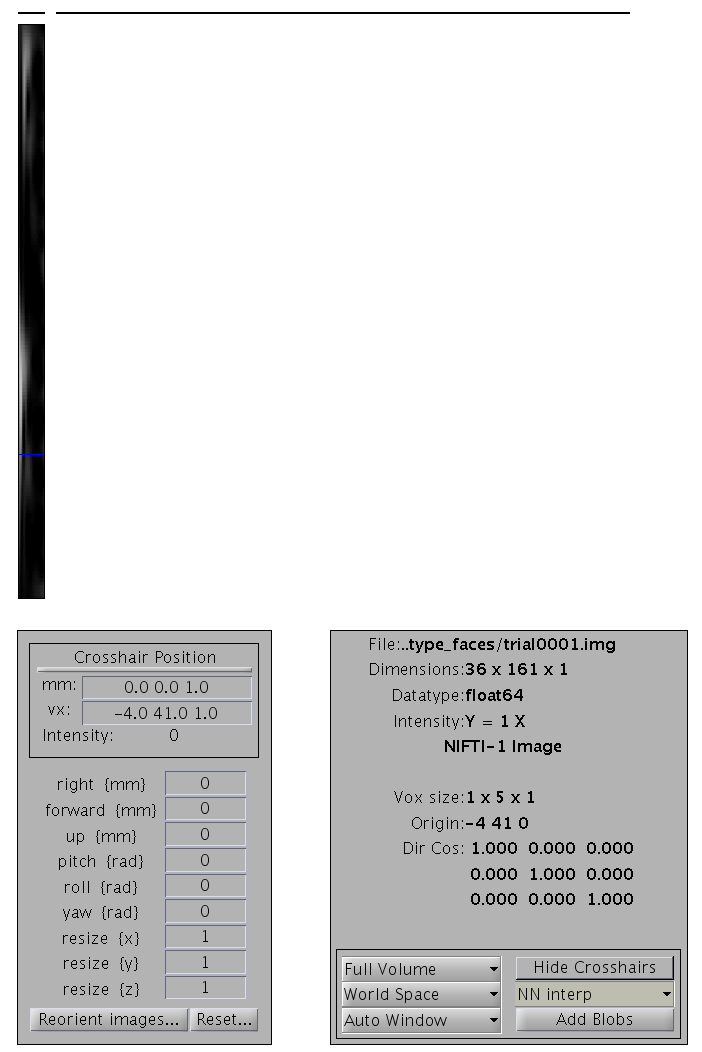
\includegraphics[width=100mm]{multimodal/figures/meg_TFimage}
\caption{\em  3D image for trial 2 within \texttt{1ROI\_TF\_trialtype\_faces} subdirectory. The bottom left section is through frequency (x) and time (y) (the other images are strips because there is only one value in the z dimension, i.e, this is really a 2D image).\label{multimodal:fig:15}}
\end{center}
\end{figure}

As in Section~\ref{multimodal:eeg:3Dsmooth}, these images can be further smoothed in time and frequency if desired. 

Then as in Section~\ref{multimodal:eeg:3DSPM}, we then take these images into an unpaired t-test across trials to compare faces versus scrambled faces. We can then use classical SPM to identify times and frequencies in which a reliable difference occurs, correcting across the multiple comparisons entailed (Kilner et al, 2005).

First create a new directory, eg. \texttt{mkdir TFstatsPow}.

Then press the \textsc{specify 2nd level} button, select ``two-sample t-test'' (unpaired t-test), and define the images for ``group 1'' as all those in the subdirectory \texttt{trialtype\_faces} (using right click, and ``select all'') and the images for ``group 2'' as all those in the subdirectory \texttt{trialtype\_scrambled}. Finally, specify the new \texttt{TFstatsPow} directory as the output directory. (Note that this will be faster if you saved and could load an SPM job file from Section~\ref{multimodal:eeg:3DSPM} in order to just change the input files and output directory.) Then add an ``Estimate'' module from the ``SPM'' tab, and select the output from the previous factorial design specification stage as the dependency input. Press ``Run'' (green arrow button).

Press \textsc{Results} and define a new T-contrast as $[1\: -1]$. Keep the default contrast options, but threshold at $p<.05$ FWE corrected for the whole search volume, and then select ``Time-Frequency'' for the ``Data Type''. Then press ``whole brain'', and the Graphics window should now look like that in Figure~\ref{multimodal:fig:16}.

\begin{figure}
\begin{center}
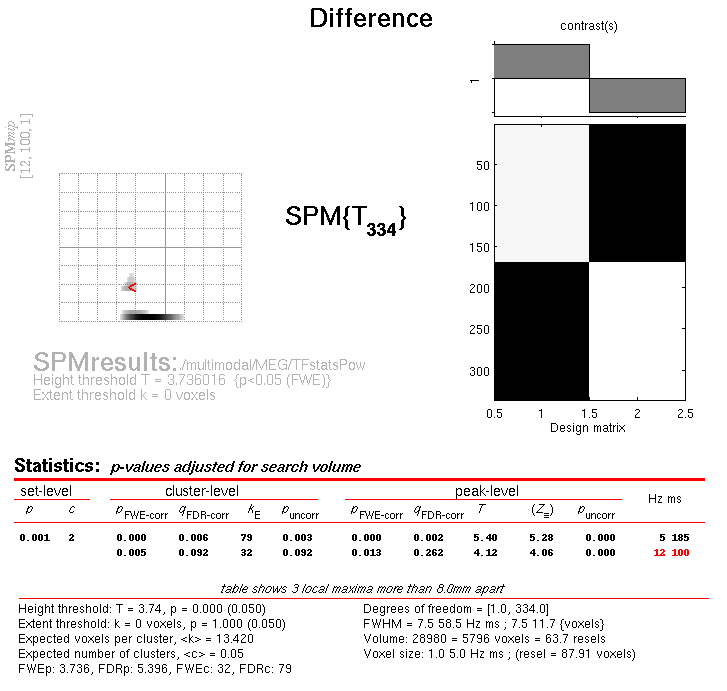
\includegraphics[width=100mm]{multimodal/figures/meg_TF_results}
\caption{\em 2D time-frequency SPM{T} at $p<.05$ FWE-corrected for the power difference between face and scrambled faces at Channel MLT34.\label{multimodal:fig:16}}
\end{center}
\end{figure}

This will list two ``regions'' within the 2D time-frequency space in which faces produce greater power than scrambled faces, having corrected for multiple T-tests across pixels. The larger one has a maximum at 5 Hz and 185 ms post-stimulus, corresponding to the M170 seen earlier in the averaged files (but now with a statistical test of its significance, in terms of evoked and induced power). The second, smaller region has a maximum at 12 Hz and 100 ms, possibly corresponding to a smaller but earlier effect on the M100 (also sometimes reported, depending on what faces are contrasted with).

\subsection{``Imaging'' reconstruction of total power for each condition \label{multimodal:data:meg:recon_pow}}

In Section~\ref{multimodal:eeg:3D} we localised the differential evoked potential difference in EEG data corresponding to the N170.  Here we will localise the total power of faces, and of scrambled faces, ie including potential induced components (see Friston et al, 2006).

Press the ``3D source reconstruction'' button, and press the ``load'' button at the top of the new window. Select the \texttt{cdbespm8\_SPM\_CTF\_MEG\_example\_faces1\_3D.mat} file and type a label (eg \texttt{M170}) for this analysis.

Press the ``MRI'' button, select the \texttt{smri.img} file within the \texttt{sMRI} sub-directory and select the ``normal'' mesh.

If you have not used this MRI image for source reconstruction before, this step will take some time while the MRI is segmented and the deformation parameters computed (see Section~\ref{multimodal:eeg:3D} for more details on these files). When meshing has finished, the cortex (blue), inner skull (red) and scalp (orange) meshes will also be shown in the Graphics window with slices from the sMRI image. This makes it possible to verify that the meshes indeed fit the original image well. The field \texttt{D.inv\{1\}.mesh} will be updated. Press ``save'' in top right of window to update the corresponding mat file on disk.

Both the cortical mesh and the skull and scalp meshes are not created directly from the segmented MRI, but rather are determined from template meshes in MNI space via inverse spatial normalisation (Mattout et al, 2007; Henson et al, 2009a).

Press the ``Co-register'' button. You will be asked for each of the 3 fiducial points to specify its location on the MRI images. This can be done by selecting a corresponding point from a hard-coded list (``select''). These points are inverse transformed for each individual image using the same deformation field that is used to create the meshes. The other two options are typing the MNI coordinates for each point (``type'') or clicking on the corresponding point in the image (``click''). Here, we will type coordinates based on where the experimenter defined the fiducials on the \texttt{smri.img}. These coordinates can be found in the \texttt{smri\_fid.txt} file also provided. So press ``type'' and for ``nas'', enter [0  91  -28]; for ``lpa'' press ``type'' and enter [-72   4  -59]; for ``rpa'' press ``type'' and enter [71  -6  -62]. Finally, answer ``no'' to ``Use headshape points?'' (see EEG Section~\ref{multimodal:eeg:3D}).

This stage coregisters the MEG sensor positions with the structural MRI and cortical mesh, via an approximate matching of the fiducials in the two spaces, followed by a more accurate surface-matching routine that fits the head-shape function (measured by Polhemus) to the scalp that was created in the previous meshing stage via segmentation of the MRI. When coregistration has finished, the field \texttt{D.inv\{1\}}.datareg will be updated. Press ``save'' in top right of window to update the corresponding mat file on disk. With the \matlab\ Rotation tool on (from the ``Tools'' tab in the SPM Graphics window, if not already on), right click near the top image and select ``Go to X-Z'' view. This should produce a figure like that in Figure~\ref{multimodal:fig:17}, which you can rotate with the mouse to check all sensors. Note that the data are in head space (not MNI space), in this case corresponding to the Polhemus space in which the X and Y dimensions are swapped relative to MNI space.

\begin{figure}
\begin{center}
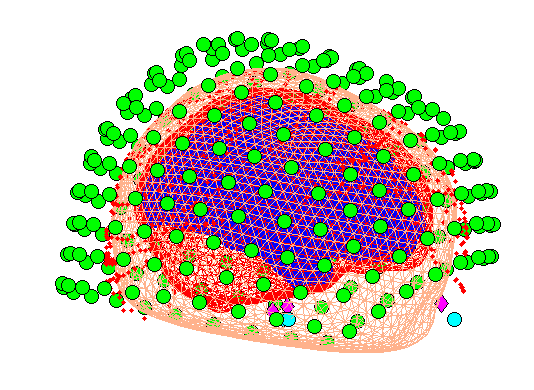
\includegraphics[width=70mm]{multimodal/figures/meg_coreg.png}
\caption{\em  Graphical output of registration of MEG and sMRI data, showing (upper panel) cortex (blue) and scalp (black) meshes, sensor locations (green), MRI and Polhemus fiducials (cyan/magneta), and headshape (red dots).\label{multimodal:fig:17}}
\end{center}
\end{figure}

Press the ``Forward Model'' button. Choose ``Local Spheres'' (you may also try the other options; see Henson et al, 2009a). A figure will be displaying showing the local (overlapping) spheres fit to each sensor, and final the set of all spheres.

Press ``Invert'', select ``Imaging'', select ``yes'' to ``All conditions or trials?'', and ``Standard'' for the model (i.e, to use defaults; you can customise a number of options if you press Custom instead) (see Friston et al, 2008, for more details about these parameters). There will be lead field computation followed by the actual inversion. A summary plot of the results will be displayed at the end.

You can now explore the results via the 3D reconstruction window. If you type 180 into the box in the bottom right (corresponding to the time in ms) and press ``mip'', you should see several ventral temporal hotspots, as in Figure~\ref{multimodal:fig:18}. Note that this localisation is different from the previous EEG localisation because 1) condition 1 now refers to faces, not the difference between faces and scrambled faces, and 2) the results reflect total power (across trials), induced and evoked, rather than purely evoked\footnote{Though in reality, most of the power is low-frequency and evoked}. The timecourses come from the peak voxel (with little evidence of a face/scrambled difference for this particular maximum). The red curve shows the condition currently being shown (corresponding to the ``Condition 1'' toggle bar in the reconstruction window); the grey curve(s) will show all other conditions. If you press the "condition 1" toggle, it will change to Condition 2, which is the total power for scrambled faces, then press ``mip'' again and the display will update (note the colours of the lines have now reversed from before, with red now corresponding to scrambled faces).

\begin{figure}
\begin{center}
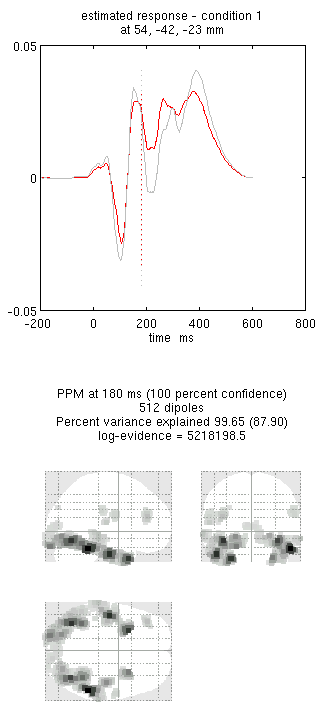
\includegraphics[width=90mm]{multimodal/figures/meg_msp.png}
\caption{\em  Graphic output for MSP-estimated activity at 159ms for faces.\label{multimodal:fig:18}}
\end{center}
\end{figure}


If press ``movie'', you will see the changes in the source strengths over peristimulus time (from the limits 0 to 300ms currently chosen by default).

If you press ``render'' you can get a very neat graphical interface to explore the data (the buttons are fairly self-explanatory). 

You can also explore the other inversion options, like COH and IID, which you will note give more superficial solutions (a known problem with standard minimum norm; see also Friston et al, 2008; Henson et al, 2009a). To do this quickly (without repeating the MRI segmentation, coregistration and forward modelling), press the ``new'' button in the reconstruction window, which by default will copy these parts from the previous reconstruction. 

In the following we will concentrate on how one prepares this single subject data for subsequent entry into a group analysis.

Press the ``Window'' button in the reconstruction window, enter ``150 200'' as the timewindow of interest and ``5 15'' as the frequency band of interest (from the SPM time-frequency analysis, at least from one channel). Then choose the ``induced'' option. After a delay (as SPM calculates the power across all trials) the Graphics window will show the mean activity for this time/frequency contrast (for faces alone, assuming the condition toggle is showing ``condition 1'').

If you then press ``Image'', press ``12'' for the smoothing kernel, and SPM will write 3D NIfTI images corresponding to the above contrast for each condition:

\begin{verbatim}
    w_cdbespm8_SPM_CTF_MEG_example_faces1_3D_1_1.nii
    w_cdbespm8_SPM_CTF_MEG_example_faces1_3D_1_2.nii
    sw_cdbespm8_SPM_CTF_MEG_example_faces1_3D_1_1.nii
    sw_ecdbespm8_SPM_CTF_MEG_example_faces1_3D_1_2.nii
\end{verbatim}

Note that the first two images are unsmoothed (but normalised); the latter two are smoothed by a 12mm isotropic Gaussian kernel. The last number in the file name refers to the condition number; the penultimate number refers to the reconstruction number (i.e. the number in red in the reconstruction window, i.e, \texttt{D.val}, here 1).

The smoothed results for Condition 1 will also be displayed in the Graphics window, together with the normalised structural. Note that the solution image is in MNI (normalised) space, because the use of a canonical mesh provides us with a mapping between the cortex mesh in native space and the corresponding MNI space.

You can also of course view the image with the normal SPM ``Display:image'' option, and locate the coordinates of the ``hotspots'' in MNI space. Note that these images contain RMS (unsigned) source estimates (see Henson et al, 2007).

If you want to see where activity (in this time/freq contrast) is greater for faces and scrambled faces, you can use SPM \texttt{ImCalc} facility to create a difference image of \texttt{sw\_\-cdbespm8\_\-SPM\_\-CTF\_\-MEG\_\-example\_\-faces1\_\-3D\_\-1\_\-1.nii} - \texttt{sw\_\-cdbespm8\_\-SPM\_\-CTF\_\-MEG\_\-example\_\-faces1\_\-3D\_\-1\_\-2.nii}: you should see bilateral fusiform. For further discussion of localising a differential effect (as in Section~\ref{multimodal:eeg:3D} with ERPs), vs taking the difference of two localisations, as here, see Henson et al (2007). The above images can then be used at the second level (assuming one also has data from other subjects) to look for effects that are consistent over a group of subjects.



\section{fMRI analysis \label{multimodal:data:fMRI}}

Only the main characteristics of the fMRI analysis are described below; for a more detailed demonstration of fMRI analysis, read previous tutorial chapters describing fMRI analyses.

Toggle the modality from EEG to fMRI, and change directory to the fMRI subdirectory (either in \matlab\, or via the ``CD'' option in the SPM ``Utils'' menu)

\subsection{Preprocessing the fMRI data}

Press the \textsc{Batch} button and then:

\begin{itemize}
\item Select \textsc{Spatial: Realign: Estimate \& Reslice} from the SPM menu, create two sessions, and select the 390 \texttt{fM*.img} EPI images within the corresponding Session1 / Session 2 subdirectories (you can use the filter  \texttt{\textasciicircum fM.*}). In the ``Resliced images'' option, choose ``Mean Image Only''.

\item Add a \textsc{Spatial: Coreg: Estimate} module, and select the \texttt{smri.img} image in the \texttt{sMRI} directory for the ``Reference Image'' and select a ``Dependency'' for the ``Source Image'', which is the Mean image produced by the previous Realign module. For the ``Other Images'', select a ``Dependency'' which are the realigned images (two sessions) from Realign.

\item Add a \textsc{Spatial: Segment} module, and select the \texttt{smri.img} image as the ``Data''.

\item Add a \textsc{Spatial: Normalise: Write} module, make a ``New: Subject'', and for the ``Parameter File'', select a ``Dependency'' of the ``Deformation Field Subj-$>$MNI'' (from the prior segmentation module). For the ``Images to Write'', select a ``Dependency'' of the ``Coreg: Estimate: Coregistered Images'' (which will be all the coregistered EPI images) and ``Segment: Bias Corr Images'' (which will be the bias-corrected structural image). Also, change the ``Voxel sizes'' to [3 3 3], to save diskspace.

\item Add a \textsc{Spatial: Smooth} module, and for ``Images to Smooth'', select a ``Dependency'' of ``Normalise: Write: Normalised Images (Subj 1)''.

\item Save the batch file (e.g, as \texttt{batch\_fmri\_preproc.mat}, and then press the ``Run'' button.
\end{itemize}

These steps will take a while, and SPM will output some postscript files with the movement parameters and the coregistration results (see earlier chapters for further explanation). The result will be a series of 2 sets of 390 \texttt{swf*.img} files that will be the data for the following 1st-level fMRI timeseries analysis.

\subsection{Statistical analysis of fMRI data}

First make a new directory for the stats output, e.g, a \texttt{Stats} subdirectory within the fMRI directory.

Press the \textsc{batch} button and then:

\begin{itemize}

\item Select ``Stats: fMRI model specification'' from the SPM module menu, and select the new \texttt{Stats} subdirectory as the ``Directory''.

\item Select ``Scans'' for ``Units of design''.

\item Enter \texttt{2} for the ``Interscan interval'' (i.e, a 2s TR).

\item Create a new session from the ``Data \& Design'' menu. For ``Scans'', select all the \texttt{swf*.img} files from the \texttt{Session1} subdirectory (except the mean). Under ``Multiple Conditions'', click ``Select File'', and select the \texttt{trials\_ses1.mat} file that is provided with these data. (This file just contains the onsets, durations and names of every event within each session.). For ``Multiple regressors'', click ``Select File'', and select the \texttt{rp*.txt} file that is also in the \texttt{Session1} subdirectory (created during realignment).

\item Repeat the above steps for the second session.

\item Under ``Basis Functions'', ''Canonical HRF'' add the ``Time and Dispersion'' derivatives.

\item Then add a ``Stats: Model estimation'' module, and for the ``Select SPM.mat'', choose the ``Dependency'' of the \texttt{SPM.mat} file from the previous ``fMRI model specification'' module.

\item Add a ``Stats: Contrast Manager'' module, and for the ``Select SPM.mat'', choose the ``Dependency'' of the \texttt{SPM.mat} file from the previous ``Model Estimation module''.

\item Under ``Contrast Sessions'', create a new F-contrast with a ``Name'' like \texttt{faces vs scrambled (all BFs)} and then enter  \texttt{[eye(3) -eye(3) zeros(3,6)]}. This will produce a 3x12 matrix that picks out the three basis functions per condition (each as a separate row), summing across the two conditions (with zeros for the movement parameter regressors, which are of no interest). Then select ``Replicate (average over sessions)''.

\item Under ``Contrast Sessions'', create a new F-contrast with a ``Name'' like \texttt{faces + scrambled vs Baseline (all BFs)} and then enter the \matlab \texttt{[eye(3) eye(3) zeros(3,6)]}. Again, select ``Replicate (average over sessions)''.

\item Save the batch file (e.g, as \texttt{batch\_fmri\_stats.mat}, and then press the ``Run'' button.

\end{itemize}

When this has finished, press \textsc{Results} and select the \texttt{SPM.mat} file that should have been created in the new \texttt{Stats} directory. The Contrast Manager window will appear, and you can select the ``faces vs scrambled (all BFs)'' contrast. Do not mask, keep the title, threshold at $p<.05$ FWE corrected, use an extent threshold of 60 voxels, and you should get the MIP and table of values (once you have pressed ``whole brain'') like that in Figure ~\ref{multimodal:fig:22}. This shows clusters in bilateral midfusiform (FFA), right occipital (OFA), right superior temporal gyrus/sulcus (STS), in addition to posterior cingulate and anterior medial prefrontal cortex. These clusters show a reliable difference in the evoked BOLD response to faces compared with scrambled faces that can be captured within the ``signal space'' spanned by the canonical HRF and its temporal and dispersion derivatives. Note that this F-contrast can include regions that show both increased and decreased amplitude of the fitted HRF for faces relative to scrambled faces (though if you plot the ``faces vs scrambled'' contrast estimates, you will see that the leftmost bar (canonical HRF) is positive for all the clusters, suggesting greater neural activity for faces than scrambled faces (also apparent if you plot the event-related responses)).

There is some agreement between these fMRI effects and the localisation of the differential ERP for faces vs scrambled faces in the EEG data (see earlier section). Note however that the fMRI BOLD response reflects the integrated neural activity over several seconds, so some of the BOLD differences could arise from neural differences outside the 0-600ms epoch localised in the EEG data (there are of course other reasons too for differences in the two localisations; see, eg, Henson et al, under revision).

\begin{figure}
\begin{center}
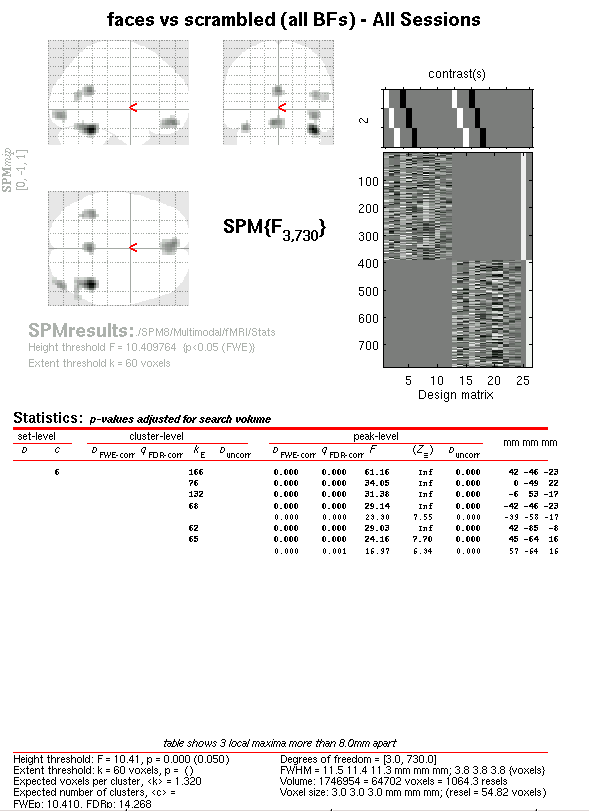
\includegraphics[width=150mm]{multimodal/figures/fmri_faces_vs_scrambled}
\caption{\em  SPM\{F\} for faces vs scrambled faces.\label{multimodal:fig:22}}
\end{center}
\end{figure}

You can also press \textsc{Results} and select the ``faces + scrambled vs Baseline (all BFs)'' contrast. Using the same threshold of $p<.05$ FWE corrected, you should see a large swathe of activity over most of the occipital, parietal and motor cortices, reflecting the general visuomotor requirements of the task (relative to interstimulus fixation). The more posterior ventral occipital/temporal BOLD responses are consistent with the MEG localisation of faces (or scrambled faces) versus baseline, though note that the more anterior ventral temporal activity in the MEG localisation is not present in the fMRI data, which suggests (but does not imply) that the MEG localisation may be erroneous.

These contrasts of fMRI data can now be used as spatial priors to aid the localisation of EEG and/or MEG data, as in the next section.


\section{Multimodal fusion\label{multimodal:fusion}}

Here, we will illustrate here two types of multimodal integration:
\begin{enumerate}
 \item ``Fusion'' of the EEG and MEG data (Henson et al, 2009b),
 \item Use of the fMRI data as spatial priors on the MEG/EEG data (Henson et al, in press).
\end{enumerate}

\subsection{EEG and MEG fusion \label{multimodal:fusion:eegmeg:fusion}}

Make a new directory called ``Fused', and change into it.

\subsubsection{Merging the EEG and MEG datafiles \label{multimodal:fusion:eegmeg:merge}}

The first step is to combine the MEG and EEG data into a single SPM file. We will use the (weighted) averaged files for each modality.

Press ``Fuse'' from the ``Others'' pulldown menu, and select the \texttt{wmcdbespm8\_\-SPM\_\-CTF\_\-MEG\_\-example\_\-faces1\_\-3D.mat} in the MEG directory and the \texttt{wmaceMdspm8\_faces\_run1.mat} in the EEG directory. This will create a new file called \texttt{uwmcdbespm8\_\-SPM\_\-CTF\_\-MEG\_\-example\_\-faces1\_\-3D.mat} in the new Fused directory. Note that the two files need to have the same number of trials, conditions, samples, etc. Display the new file, and you will see the EEG and MEG data within their respective tabs.

We have to do one extra bit of ``preparation'' for the EEG data. Because in general, one might want to merge more than one EEG file, integrating all their locations could be tricky. So the simple answer is to clear all locations and force the user to re-specify them. So (as in earlier EEG section), select \textsc{Prepare} from the ``Other'' menu and select \texttt{uwmaceMdspm8\_faces\_run1.mat}. Then in the SPM Interactive window, on the ``Sensors'' submenu, choose ``Load EEG sensors''/``Convert locations file'', and select the \texttt{electrode\_locations\_and\_headshape.sfp} file (in the original EEG directory). Then from the ``2D projection'' submenu select ``Project 3D (EEG)''. A 2D channel layout will appear in the Graphics window. Select ``Apply'' from ``2D Projection'' and ``Save'' from ``File'' submenu.

\subsubsection{3D fused ``imaging'' reconstruction \label{multimodal:fusion:eegmeg:3D}}

Now we can demonstrate simultaneous reconstruction of the MEG and EEG data, as described in Henson et al (2009b). This essentially involves scaling each type of data and gain matrix, concatenating them, and inverting using the normal methods, but with separate sensor error covariance terms for each modality.
\begin{itemize}
\item Press the ``3D source reconstruction'' button, and load the \texttt{uwmcdbespm8\_\-SPM\_\-CTF\_\-MEG\_\-example\_\-faces1\_\-3D.mat} file. Type a label (eg ``N/M170'').

\item Press the ``MRI'' button, select the \texttt{smri.img} file within the \texttt{sMRI} sub-directory, and select ``normal'' for the cortical mesh. Because this MRI was normalised previously, this step should not take long, finishing with display of the cortex (blue), inner skull (red), outer skull (orange) and scalp (pink) meshes.

\item Press the ``Co-register'' button. Press ``type'' and for ``nas'', enter [0 91 -28] for ``lpa'' press ``type'' and enter [-72 4 -59] for ``rpa'' press ``type'' and enter [71 -6 -62]. Finally, answer ``no'' to ``Use headshape points?''. Then select either ``EEG'' or ``MEG'' to display corresponding
data registration. Note that the MEG data will have been coregistered to the EEG data in the headspace. If you want to display the other modality afterwards, just press the ``display'' button below the ``Co-register'' button.

\item Press ``Forward Model'', and select ``EEG BEM'' for the EEG and ``Local Spheres'' for the MEG. Then select either ``EEG'' or ``MEG'' to display corresponding forward model. (If you want to display the other modality afterwards, just press the ``display'' button below the ``Forward Model'' button). In the Graphics window the meshes will be displayed with the sensors marked with green asterisks.

\item Press ``save'' to save progress.

\item Press ``Invert'', select ``Imaging''. Because the fMRI data (see below) already come from a contrast of faces versus scrambled faces, we will only invert the differential ERP/ERFs. So press ``no'' to the question about invert ''all conditions or trials'', press ''yes'' to invert the Difference (between faces and scrambled) but ''no'' to invert the Mean (of faces and scrambled versus baseline). 

Then press ``Standard'' to use the default inversion settings (MSP), and then to select both the ``EEG'' and ``MEG'' modalities in the new ``Select modalities'' window, in order to fuse them (simultaneously invert both).

Lead fields will first be computed for all the mesh vertices and saved in the file \texttt{SPMgainmatrix\_uwmcdbespm8\_SPM\_CTF\_MEG\_example\_faces1\_3D\_1.mat}. 
This will take some time.
Then the actual MSP algorithm will run and the summary of the solution will be displayed in the Graphics window.

\item Press ``save'' to save the results. You can now explore the results via the 3D reconstruction window. If you type 180 into the box in the bottom right (corresponding to the time in ms) and press ``mip'', you should see an output similar to Figure~\ref{multimodal:fusion:fig:1}.
\end{itemize}

\begin{figure}
\begin{center}
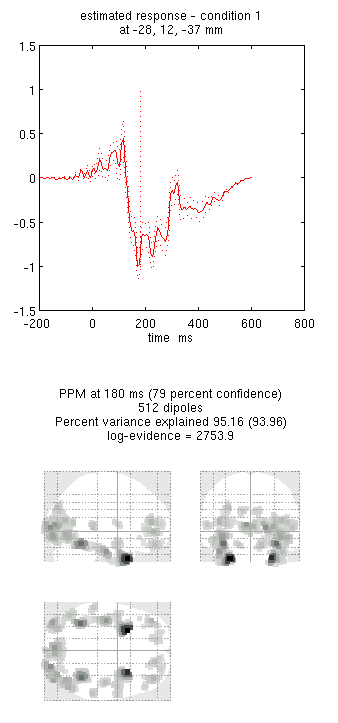
\includegraphics[width=90mm]{multimodal/figures/fused_eeg_meg_msp.png}
\caption{\em Graphical output of an MSP estimation of the differential evoked response between faces and scrambled faces at 180ms, after fusing both EEG and MEG data. \label{multimodal:fusion:fig:1}}
\end{center}
\end{figure}

Note that because we have inverted only the differential ERP/ERF, these results cannot be compared directly to the unimodal inversions in the previous sections of this chapter. For a fairer comparison:

\begin{itemize}
\item Press the ``new'' button and type ``N170'' as the label, press ``Invert'' again (note that all forward models are copied by default from the first inversion) and select the same options as above, except that when asked ``Select modalities'', select just ``EEG''. This should produce the results in Figure~\ref{multimodal:fusion:fig:2}. Notice the more posterior maxima.

\begin{figure}
\begin{center}
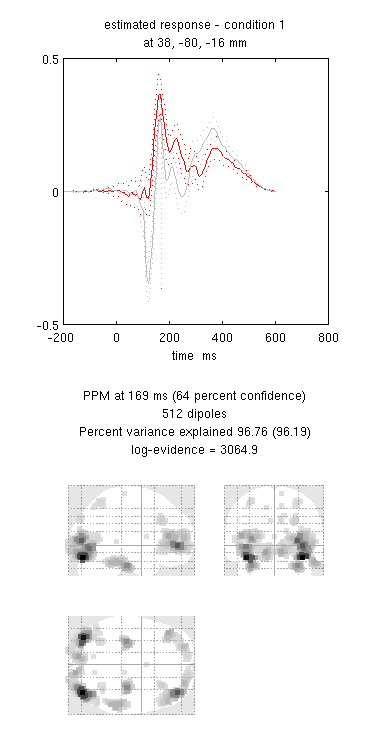
\includegraphics[width=90mm]{multimodal/figures/fused_eeg_msp.png}
\caption{\em Graphical output of an MSP estimation of the differential evoked response between faces and scrambled faces at 180ms, after inverting just EEG data. \label{multimodal:fusion:fig:2}}
\end{center}
\end{figure}

\item Press the ``new'' button and type ``M170'' as the label, press ``Invert'' again and select the same options as above, except that when asked ``Select modalities'', select just ``MEG'' this time. This should produce the results in Figure~\ref{multimodal:fusion:fig:3}. Notice the more anterior and medial activity.

\begin{figure}
\begin{center}
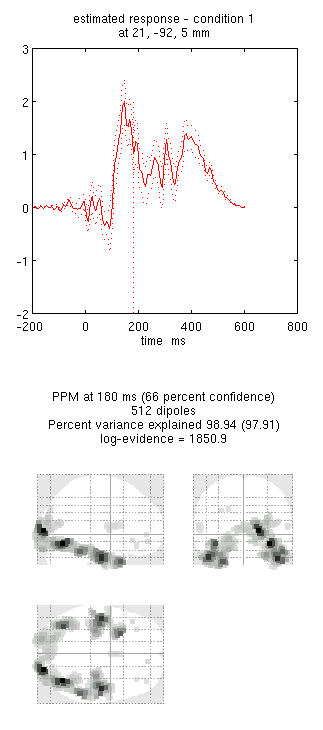
\includegraphics[width=90mm]{multimodal/figures/fused_meg_msp.png}
\caption{\em Graphical output of an MSP estimation of the differential evoked response between faces and scrambled faces at 180ms, after inverting just MEG data. \label{multimodal:fusion:fig:3}}
\end{center}
\end{figure}

\end{itemize}

By comparing these figures, you can see that the multimodal fused inversion (first inversion) combines aspects of both the unimodal inversions. Unfortunately one cannot simply compare the multi-modal vs uni-modal reconstructions via the log-evidence, because the data differs in each case (rather, one could use an estimate of the conditional precision of the sources, as in Henson et al, 2009b). With multiple subjects though, one could compare statistics across subjects using either multimodal or unimodal inversions.

\subsection{EEG, MEG and fMRI fusion \label{multimodal:fusion:fmri}}

Now we can examine the effects of using the fMRI data in Section~\ref{multimodal:data:fMRI} as spatial priors on the sources (Henson et al, in press). But first we need to create an 3D volumetric image of the clusters that we wish to use as spatial priors. These clusters can be defined by thresholding an SPM for a given fMRI contrast: here we will use the contrast in Section~\ref{multimodal:data:fMRI} of faces versus scrambled faces (using all three basis functions). So press ``Results'' and select the ``SPM.mat'' file from the ``fMRI/Stats'' directory. Select the previous faces vs scrambled F-contrast, do not mask or change title, use FWE correction at 0.05 and a 60-voxel extent to reproduce the SPM\{F\} shown in Figure~\ref{multimodal:fig:22} (if you are still in SPM's ``EEG'' mode, you will also be asked the type of images, for which you reply ``Volumetric 2D/3D'').

Now press the ``save'' button in the Interactive window and enter a filename like \texttt{Faces\-Vs\-Scrambled\_FWE05\_60}. This will produce a 3D image (which you can display as normal) in which all subthreshold voxels are set to zero (ie, where only 6 clusters containing non-zero voxel values are left).

Now we can use this cluster image in a new inversion:

\begin{itemize}

\item Press the ``new'' button to create a fourth inversion, and type ``N/M170+fMRI'' as the label.

\item Press ``Invert'', select ``Imaging'', press ''no'' for ''all conditions or trials'', and select only the Difference (not Mean), as before ...

\item ... but this time, press ``Custom'' rather than ``Standard'' to get more flexibility in the inversion settings. Select ``GS'' for the type of inversion (the default MSP with a Greedy Search), enter default time window of ``-200 to 600'', ``yes'' to a Hanning window, ``0'' for the highpass and ``48'' for the lowpass, and then press ``yes'' to the question of ``Source priors?''...

\item ... select the \texttt{FacesVsScrambled\_\-FWE05\_\-60.img} file in the ``fMRI/Stats'' directory, and select ``MNI'' for the ``Image space'' (because the fMRI images were spatially normalised).

\item Say ``No'' to ``Restrict solutions'', and then select both the ``EEG'' and ``MEG'' modalities in the ``Select modalities'' window, in order to fuse them (together with the fMRI priors).

Note that, once the inversion has finished, a new image will be created (in the ``fMRI/Stats'' directory) called \texttt{cluster\_\-FacesVsScrambled\_\-FWE05\_\-60.img}, which contains the six binary priors, as will a GIfTI version called \texttt{priors\_\-uwmcdbespm8\_\-SPM\_\-CTF\_\-MEG\_\-example\_\-faces1\_\-3D\_\-4.func.gii}. If you want to display each spatial prior on the cortical mesh, first make sure you save the current reconstruction, and then type in the \matlab\ window: 

\begin{verbatim}
  D = spm_eeg_load('uwmcdbespm8_SPM_CTF_MEG_example_faces1_3D.mat');
  val = 4;    % Fourth inversion; assuming you have followed the above steps
  G = gifti(D.inv{val}.mesh.tess_mni);
  P = gifti(D.inv{val}.inverse.fmri.texture);
  for i=1:size(P.cdata,2);
    figure, plot(G,P,i);
  end
\end{verbatim}

Finally, a new \matlab\ file called \texttt{priors\_\-uwmcdbespm8\_\-SPM\_\-CTF\_\-MEG\_\-example\_\-faces1\_\-3D\_\-4.mat} will also be saved to the current directory, which contains the information necessary to construct the covariance components for subsequent inversion. So if you want to use these fMRI priors in another inversion, next time you are prompted for the ``Source priors?'', rather than selecting an image (``img'' file) as we did above, you can select this ``mat'' file, so SPM will not need to recreate the covariance matrices from the image file, but can use the covariance matrices directly.

\item Again, type 180 into the box in the bottom right and press ``mip''. This should produce the output in Figure~\ref{multimodal:fusion:fig:4}.  Notice how the more posterior midfusion clusters (particularly on the left) have become stronger (where there were fMRI priors). (Note also that fMRI priors have generally been found to have a greater effect on IID or COH inversions, given the implicit flexibility of MSP priors, Henson et al, in press).

\begin{figure}
\begin{center}
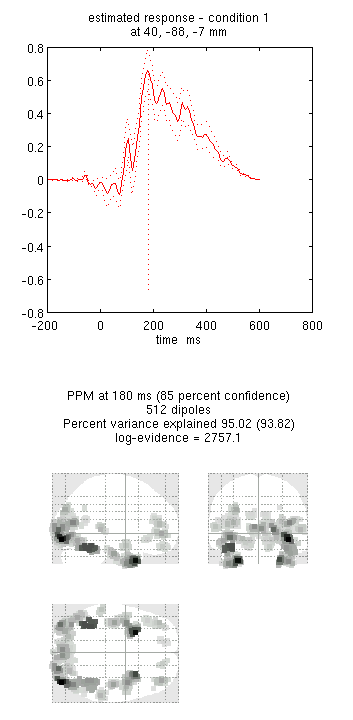
\includegraphics[width=90mm]{multimodal/figures/fused_eeg_meg_msp_fmri.png}
\caption{\em Graphical output of an MSP estimation of the differential evoked response between faces and scrambled faces at 180ms, after fusing EEG, MEG and fMRI data. \label{multimodal:fusion:fig:4}}
\end{center}
\end{figure}


\item Press ``save''.

\end{itemize}

You can repeat the above steps to use the common fMRI effect of faces and scrambled faces versus baseline (though at a higher threshold perhaps) as an alternative set of spatial priors for inverting either the differential evoked MEG/EEG response, or the mean evoked MEG/EEG response vs baseline. 



\section{References}

\noindent 1. Friston, K, Daunizeau, J, Kiebel, S, Phillips, C, Trujillo-Barreto, N, Henson, R, Flandin, G, Mattout, J (2008). Multiple sparse priors for the M/EEG inverse problem. Neuroimage, 39(3):1104-20.\\

\noindent 2. Friston, K, Carlton Chu, Janaina Mouro-Miranda, Oliver Hulme, Geraint Rees, Will Penny and John Ashburner (2008). Bayesian decoding of brain images. NeuroImage, 39(1):181-205.\\

\noindent 3. Friston K, Henson R, Phillips C, and Mattout J. (2006). Bayesian estimation of evoked and induced responses. Human Brain Mapping, 27, 722-735.\\

\noindent 4. Henson, R, Goshen-Gottstein, Y, Ganel, T, Otten, L, Quayle, A. and Rugg, M. (2003). Electrophysiological and hemodynamic correlates of face perception, recognition and priming. Cerebral Cortex, 13, 793-805.\\

\noindent 5. Henson R, Mattout J, Friston K, Hassel S, Hillebrand A, Barnes G and Singh K. (2005a) Distributed source localisation of the M170 using multiple constraints. HBM05 Abstract.\\

\noindent 6. Henson R, Kiebel S, Kilner J, Friston K, Hillebrand A, Barnes G and Singh K. (2005b) Time-frequency SPMs for MEG data on face perception: Power changes and phase-locking. HBM05 Abstract.\\

\noindent 7. Henson, R, Mattout, J, Singh, K, Barnes, G, Hillebrand, A and Friston, K.J. (2007). Population-level inferences for distributed MEG source localisation under multiple constraints: Application to face-evoked fields. Neuroimage, 38, 422-438.\\

\noindent 8. Henson, R, Mattout, J, Phillips, C and Friston, K.J. (2009a). Selecting forward models for MEG source-reconstruction using model-evidence. Neuroimage, 46, 168-176.\\

\noindent 9. Henson, R, Mouchlianitis, E and Friston, K.J. (2009b). MEG and EEG data fusion: Simultaneous localisation of face-evoked responses. Neuroimage, 47, 581-589.\\

\noindent 10. Henson, R, Flandin, G, Friston, K.J. and Mattout, J. (in press). A Parametric Empirical Bayesian framework for fMRI-constrained MEG/EEG source reconstruction. Human Brain Mapping.\\

\noindent 11. Kilner, J., Kiebel, S and Friston, K. J. (2005). Applications of random field theory to electrophysiology. Neuroscience Letters, 374:174-178.\\

\noindent 12. Kilner, J. and Penny. W. (2006). Robust Averaging for EEG/MEG. HBM06 Abstract.\\

\noindent 13. Kiebel S and Friston K (2004). Statistical Parametric Mapping for Event-Related Potentials II: A Hierarchical Temporal Model. NeuroImage, 22, 503-520.\\

\noindent 14. Kiebel, S.J., David, O. and Friston, K. J. (2006). Dynamic Causal Modelling of Evoked Responses in EEG/MEG with lead-field parameterization. NeuroImage, 30:1273-1284.\\

\noindent 15. Mattout J, Pelegrini-Issac M, Garnero L and Benali H. (2005a). Multivariate source prelocalization (MSP): use of functionally informed basis functions for better conditioning the MEG inverse problem. Neuroimage, 26, 356-73.\\

\noindent 16. Mattout, J, Phillips, C, Penny, W, Rugg, M and Friston, KJ (2005b). MEG source localisation under multiple constraints: an extended Bayesian framework. NeuroImage.\\

\noindent 17. Mattout, J., Henson, R N. and Friston, K.J. (in press). Canonical Source Reconstruction for MEG. Computational Intelligence and Neuroscience.\\

\noindent 18. Phillips, C, M.D. Rugg, M and Friston, K.J. (2002). Systematic Regularization of Linear Inverse Solutions of the EEG Source Localisation Problem. NeuroImage, 17, 287-301.\\

\noindent 19. Spinelli, L, Gonzalez S, Lantz, G, Seeck, M and Michel, C. (2000). Electromagnetic inverse solutions in anatomically constrained spherical head models. Brain Topography, 13, 2.\\

\noindent 20. Wager, TD, Keller, MC, Lacey SC and Jonides J. (2005). Increased sensitivity in neuroimaging analyses using robust regression. NeuroImage, 26(1), 99-113.\\
